\documentclass{article}
\usepackage[utf8]{inputenc}
\usepackage[serif]{lindrew}
\usepackage{cancel}
\usepackage{pgf, tikz}
\usepackage{pdfpages}
\usepackage{mathdots}
\usepackage{subcaption}
\usetikzlibrary{arrows, automata}
\usepackage{upgreek}
\usepackage{amsmath, amssymb}
\usepackage{graphicx}
\usepackage{wrapfig}
\usepackage{fontspec,xeCJK}
\usepackage{ctex}
\usepackage[yyyymmdd]{datetime}
% change to frozencache for uploading to arXiv, and include the _minted files in the arXiv submission
\usepackage[frozencache,cachedir=_minted]{minted}
\setCJKmainfont[Path=./fonts/]{simkai.ttf}
\setCJKsansfont[Path=./fonts/]{STZHONGS.ttf} % 设置无衬线字体为 华文中宋
\setCJKmonofont[Path=./fonts/]{simkai.ttf} % 设置等宽字体为 KaiTi
\setlength{\parindent}{0pt} % 取消缩进
\usepackage{enumitem}
\setenumerate[1]{itemsep=0pt,partopsep=0pt,parsep=\parskip,topsep=5pt}
\setitemize[1]{itemsep=0pt,partopsep=0pt,parsep=\parskip,topsep=5pt}
\setdescription{itemsep=0pt,partopsep=0pt,parsep=\parskip,topsep=5pt}

%\usepackage{todonotes}
\newcommand{\todo}[1]{}

\title{随机过程}
\author{\textbf{教授:吴明燕} \\ 笔记由Dafu Zhu编写 \\ 基于2025春季厦大数院《随机过程》}

\renewcommand{\d}{d}
\newcommand{\diag}{\operatorname{diag}}
\newcommand{\cofactor}{\mathrm{cofactor}}
\newcommand{\adj}{\operatorname{adj}}
\newcommand{\vecm}{\operatorname{vec}}
\newcommand{\dotstar}{\mathbin{.*}}
\newcommand{\evalat}[2]{\left. #1 \right|_{#2}}
\newcommand{\red}[1]{\textcolor{red}{#1}}

\usepackage{kbordermatrix}
\renewcommand{\kbldelim}{(} % change array delimiters to (...)
\renewcommand{\kbrdelim}{)}

\newcommand{\alan}[1]{\textcolor{blue}{#1}}

\date{最后修改:\today}

\begin{document}

\maketitle

\tableofcontents

\pagebreak

\section{概率论准备知识}
成绩:平时(作业+考勤)+期中论文+期末

\section*{概率论准备知识}

概率论中,随机变量的本质是可测函数。

\[
X:\Omega\rightarrow S
\]

$S$ 的 $\sigma$-代数记为 $\mathcal{S}$,是个 Borel $\sigma$-代数(由开集/闭集生成)

Q: 为什么要给 $\Omega$ 一个$\sigma$-代数?

A: 样本空间是抽象的,给它$\sigma$-代数赋予它结构,相当于对信息进行重整/提取

概率测度的本质是集函数,

\[
\text{集合}\rightarrow \text{函数}
\]

将信息具象化,

\[
\begin{aligned}
    \PP: &\mathcal{F}\rightarrow [0,1]\\
    &A\rightarrow \PP(A)
\end{aligned}
\]

随机过程:一族随机变量 $\{X_t\}_{t\in \mathbb{T}}$

其中 $\mathbb{T}$ 为指标集,$X_t:\Omega\rightarrow S$

\begin{example}
$\mathbb{T}=\mathbb{N}_0$: 时间离散;$\mathbb{T}=[0,T]$: 时间连续 
\end{example}

\[
X:(\Omega, \mathcal{F}, \PP)\rightarrow (S,\mathcal{S}, \mu_X)
\]

思考:什么是随机过程的分布$\{\mu_t\}_{t\in \mathbb{T}}$?

\newpage

\subsection{事件概率}

\subsubsection{事件域}

\begin{definition}[样本空间、事件]
    样本点、样本空间、事件和事件的运算:
    \begin{itemize}
        \item 样本点 $\omega$: 一次试验的结果
        \item 样本空间 $\Omega$: 全体样本点
        \item 事件:$\Omega$ 的子集
        \item 事件的运算:集合的运算,即交并补($A\cap B, A\cup B, A^c$)
    \end{itemize}
\end{definition}

\begin{definition}
    若 $A\cap B=\varnothing$,则称 $A$ 与 $B$ 不相交,更一般地,若 $A_i\cap A_j=\varnothing (i\neq j)$,则称 $\{A_i\}_{i\geq 1}$ 互不相交
\end{definition}

\begin{definition}[$\sigma$-代数]
    称 $\mathcal{F}\subset 2^{\Omega}=\{A|A\subset \Omega\}$ 是一个 $\sigma$-代数/事件域(其中 $2^{\Omega}$ 表示所有 $\Omega$ 的子集构成的集合,是一个集类)

    若\begin{enumerate}
        \item $\Omega\subset \mathcal{F}$
        \item (对补封闭) $A\in \mathcal{F}\rightarrow A^c\in \mathcal{F}$
        \item (对可列并封闭) $A_n\in \mathcal{F}, n\geq 1\Rightarrow \cup_{n\geq 1}A_n=\cup_{n=1}^{\infty} A_n\in\mathcal{F}$
    \end{enumerate}

    $\sigma$代数是满足以上特定条件的集类,是由 $\Omega$ 的子集构成的集合

    注:$\sigma$代数对有限交/有限并/可列交封闭
\end{definition}

现在给出了一个定义,我们会想 “为什么定义会这样给呢”,现在要举一些例子说明 “定义有意义”

\begin{example}
    最小的 $\sigma$代数:$\{\varnothing, \Omega\}$ 

    最大的 $\sigma$代数:$2^{\Omega}$
\end{example}

以上这两个例子一个太小、一个太大,似乎没意义,所以叫它们 “平凡的”

\begin{example}
    $A\subset \Omega, \sigma(\{A\})=\sigma(A)=\{A, A^c, \Omega, \varnothing\}=\sigma(A^c)$

    这是由 $A$ 生成的 $\sigma$代数
\end{example}

\begin{definition}[划分/分割]\label{def:partition}
    称 $\Pi_{\Omega}:= \{\Lambda_n, n\geq 1\}$ 是 $\Omega$ 的一个分划,若 $\Omega=\sum_{n\geq 1}\Lambda_n$

    \begin{enumerate}
        \item $\Omega=\cup_{n\geq 1}\Lambda_n$
        \item $\{\Lambda_n\}_{n\geq 1}$ 互不相交
    \end{enumerate}
\end{definition}

\begin{example}
    $\Omega=\sum_{n\geq 1}\Lambda_n, \Pi_{\Omega}:=\{\Lambda_n\}_{n\geq 1}$

    \[
    \sigma(\Pi_{\Omega})=\left \{\sum_{k\in J}\Lambda_k, J\subset \mathbb{N}\right \}
    \]
\end{example}

\begin{problem}[作业1-1]
    证明:\begin{enumerate}
        \item $\sigma(\Pi_{\Omega})$ 是一个 $\sigma$代数
        \item $\sigma(\Pi_{\Omega})$ 是包含集类 $\Pi_{\Omega}$ 的最小 $\sigma$代数
    \end{enumerate}
\end{problem}


$(S,\mathcal{S})=(S,2^S)$: S 可列时,取 $2^S$ 为 $\sigma$代数

$(S,\mathcal{S})=(\mathbb{R},\mathcal{B}(\mathbb{R}))$: S 为实数集时,取博雷尔集 $\mathcal{B}(\mathbb{R})$ 为 $\sigma$代数


\subsubsection{概率测度}

\begin{definition}[概率测度]\label{def:prob_measure}
    $(\Omega, \CF)$ 称 $\PP: \mathcal{F}\rightarrow [0,1]$ 是概率测度
    \begin{enumerate}
        \item 非负性
        \item 归一性
        \item 可列可加性*
    \end{enumerate}
    其中,可列可加性的表述为:设 $\{E_n, n\geq 1\}$ 是 $\CF$ 中互不相交的集合序列($E_i\cap E_j=\emp, i\neq j$),则
    \[
    \PP(\cup_{n=1}^{\infty}E_n)=\sum_{n=1}^{\infty}\PP(E_n)
    \]
\end{definition}

\begin{property}
$\PP$ 满足有限可加性(可列可加一定有限可加,如果既不是可列可加、也不是有限可加,则不可测)
\end{property}

\begin{corollary}\label{cor:set_operation}
    1. $\PP(A)=1-\PP(A^c)$

    2. 若 $A\subset B$,则 $\mathbb{B}=\mathbb{A}+\PP(BA^c)\geq \PP(A)$

    3. $\PP(A\cup B)=\PP(A)+\PP(B)-\PP(A\cap B)$
\end{corollary}

\begin{remark}
    引用知乎上\href{https://www.zhihu.com/question/25836213/answer/1204497999}{三维之外}的大白话解释可列可加性:

    首先,在我们总是习惯于处理有限相加,而很少遇到无限相加的情况。从测度论内容理解,有限相加与事实(数学的)不符,比如$(0,1)$区间有不可数个点,每个点的测度(理解为直径吧)是$0$,按照习惯想法(有限相加),直径的加和(总宽度)应该为$0$,显然,$(0,1)$区间的宽度不可能是$0$;
    
    如果规定为“只要是无穷多个点相加,其宽度就不再是$0$”的话,还是存在矛盾,我们知道,区间$(0,1)$上的有理数是是无穷多个的(而且是可列的),那么其宽度就应该为$1$,可是无理数还是不可数的呢——理解为无理数是有理数的无穷大量或有理数是无理数的无穷小量,那么无理数的宽度是多少呢?即使还是$1$,显然$(0,1)$区间的宽度不可能是$2$吧!?
    
    于是,勒贝格说道:在测量长度、面积、体积时,我们采用可列可加性,即可列个点相加,规定其宽度(测度)为$0$,如果点的个数超过了可列个(这时必是连续统的),那么,就不满足了——即这些点的总宽度就不是$0$了 ,而是具有了非$0$的宽度(正测度),当然,具有测度的这些点是紧挨在一起的,否则不一定有测度,比如康托大师制造的三分集就很诡异。
    
    到这里,可列可加性事实上讲完了,再啰嗦一下次可列可加性。这是因为不论作为集合,还是概率上的事件(也是集合),一般是存在公共元素的,因此,一般情形下,当然满足次可列可加性的性质了,可列可加性只有在集合之间的距离大于$0$或事件之间完全独立的情形下,才会满足。
\end{remark}

\begin{property}[次可列可加性]
    $A_n\subset \mathcal{F}, n\geq 1$

    \[
    \PP(\bigcup_{n\geq 1}A_n)\leq \sum_{n\geq 1}\PP(A_n)
    \]
\end{property}

证明:$\cup_{n\geq 1}A_n=\sum_{n\geq 1}B_n$,其中 $B_1=A_1, B_2=A_2\cap (A_1)^c,\cdots , B_n=A_n\cap A_1^c\cap A_2^c\cap \cdots \cap A_{n-1}^c$

$B_n\subset A_n$,由可列可加性和推论\ref{cor:set_operation}(2)

\begin{problem}[作业1-2]\label{exer:disjoint_union}
证明 $\cup_{n\geq 1}A_n=\sum_{n\geq 1}B_n$
\end{problem}

证明:
\begin{enumerate}
    \item 先证 \(\bigcup_{n \geqslant 1} A_n \st \sum_{n \geqslant 1} B_n\)。

    假设 \(x \in \bigcup_{n \geqslant 1} A_n\),

    若 \(x \in A_1\),则 \(x \in B_1\),

    若 \(x \in A_2\) 且 \(x \notin A_1\),则 \(x \in B_2\)

    $\cdots$

    若 \(x \in A_n\) 且 \(x \notin A_1\), \(x \notin A_2\), \(\ldots\), \(x \notin A_{n-1}\),则 \(x \in B_n\)

    $\forall x\in \bigcup_{n\geq 1}A_n$,都有 $x\in \bigcup_{n\geq 1}B_n$

    \(\because B_i \cap B_j = \emp,i\neq j\),\(\therefore \bigcup_{n \geqslant 1} B_n = \sum_{n \geqslant 1} B_n\),\(x \in \sum_{n \geqslant 1} B_n\)。

    \item 再证 \(\sum_{n \geqslant 1} B_n \st \bigcup_{n \geqslant 1} A_n\)

    假设 \(x \in \sum_{n \geqslant 1} B_n\),则 \(\exists n_0 \in \mathbb{N}^+\),使得 \(x \in B_{n_0}\),

    由$B$的定义

    \[
    B_{n_0} = A_{n_0} \cap \left( \bigcap_{k=1}^{n_0-1} A_k^c \right)
    \]

    \(\therefore x \in A_{n_0} \subseteq \bigcup_{n \geqslant 1} A_n\)

    \(\therefore \bigcup_{n \geqslant 1} A_n = \sum_{n \geqslant 1} B_n\)\qed
\end{enumerate}

\begin{property}[连续性]\label{prt:measure_continuity}
    (1) $A_n\uparrow$单调上升,即$A_n\subset A_{n+1}$,$\lim_{n\rightarrow \infty}A_n=\cup_{n\geq 1}A_n$,则 $\PP(\lim_{n\rightarrow \infty}A_n)=\lim_{n\rightarrow \infty}\PP(A_n)$

    (2) $B_n\downarrow$单调下降,即$B_n\supset B_{n+1}$,$\lim_{n\rightarrow \infty}B_n=\cap_{n\geq 1}B_n$,则 $\PP(\lim_{n\rightarrow \infty}B_n)=\lim_{n\rightarrow \infty}\PP(B_n)$
\end{property}

证明:(1) $\cup_{n\geq 1}A_n=A_1+A_2\setminus A_1+A_3\setminus A_2+\cdots$

\[
\begin{aligned}
    \PP(\bigcup_{n\geq 1}A_n)&=\PP(A_1)+\sum_{n\geq 1}\PP(A_{n+1}\setminus A_n)\\
    &=\PP(A_1)+\limit{m}\sum_{n=1}^m \PP(A_{n+1}\setminus A_n)\\
    &=\PP(A_1)+\limit{m}\sum_{n=1}^m [\PP(A_{n+1})-\PP(A_n)]\\
    &=\PP(A_1)+\limit{m}[\PP(A_{m+1})-\PP(A_1)]\\
    &=\limit{m} \PP(A_{m+1})\\
    &=\limit{n} \PP(A_n)\qed
\end{aligned}
\]

(2) $B_n\downarrow B\Rightarrow \forall n, B_{n+1}\st B_n \Rightarrow \forall B_n^c\st B_{n+1}^c$

\[
\begin{aligned}
    \PP(B) = \PP(\cap_{n\geq 1}B_n) &= 1-\PP((\cap_{n\geq 1}B_n)^c)\\
    &=1-\PP(\cup_{n\geq 1}B_n^c)\\
    &=1-\PP(B_1^c\cup (\cup_{n\geq 2}(B_n^c\setminus B_{n-1}^c)))\\
    &=1-\PP(B_1^c)-\sum_{n\geq 2}(\PP(B_n^c)-\PP(B_{n-1}^c))\\
    &=1-\PP(B_1^c)-\limit{m}\sum_{n=2}^m(\PP(B_n^c)-\PP(B_{n-1}^c))\\
    &=1-\PP(B_1^c)-\limit{m}(\PP(B_m^c)-\PP(B_1^c))\\
    &=1-\PP(B_1^c)-\limit{n}\PP(B_n^c)+\PP(B_1^c)\\
    &=1-\limit{n}\PP(B_n^c)\\
    &=\limit{n}\PP(B_n)\qed
\end{aligned}
\]

第二个等式用到De Morgan's Law

\newpage
\subsection{独立性}

\begin{definition}[事件间的独立性]
    $(\Omega,\CF, \PP), A,B\in \CF$,称 A 与 B 独立,若 $\PP(A\cap B)=\PP(A)\PP(B)$,记为 $A\ind B$
\end{definition}

\begin{definition}[事件间的相互独立]
    $\series{A}{n} \subset \CF$,称其相互独立,若 $\forall J\subset \NN, \#J\geq 2$
    \[
    \PP(\bigcap_{k\in J}A_k)=\prod_{k\in J}\PP(A_k)
    \]
\end{definition}

\begin{property}\label{prop:counter_indep}
    $A\ind B\Rightarrow A\ind B^c, A^c \ind B, A^c\ind B^c$
\end{property}

\begin{definition}[$\sigma$代数间的独立性]\label{def:sigma_indep}
    $(\Omega, \CF_1, \PP), (\Omega, \CF_2, \PP)$ 称 $\CF_1$ 与 $\CF_2$ 独立,若 $\forall A_1\in \CF_1, A_2\in \CF_2$,有 $A_1\ind A_2$,记为 $\CF_1\ind \CF_2$
\end{definition}

\begin{definition}[$\sigma$代数间相互独立]
    $(\Omega, \CF_k, \PP)(k\geq 1)$ 称 $\series{\CF}{k}$ 相互独立,若 $\forall J\subset \NN, \#J\geq 2, \forall A_k\in \CF_k(k\in J)$,有
    \[
    \PP(\bigcap_{k\in J}A_k)=\prod_{k\in J}P(A_k)
    \]
\end{definition}

\begin{property}\label{prop:equiv_sigma_mutual_indep}
    $\series{\CF}{k}$ 相互独立 $\Leftrightarrow$ $\forall A_k\in \CF_k, \PP(\cap_{k\geq 1}A_k)=\prod_{k=1}^{\infty}\PP(A_k)$
\end{property}

证明:$\Rightarrow$ 显然,$J$ 取 $\NN$ 即可,$\NN\subset \NN$

$\Leftarrow$ 注意到右侧 $\forall A_k\in \CF$ 对于左侧条件 $\forall A_k\in \CF(k\in J)$ 更加一般,所以证 $\Leftarrow$ 的过程也是从一般到特殊。从 $\cap_{k\geq 1}A_k\rightarrow \cap_{k\in J}A_k$ 即从 $k\in\NN\rightarrow k\in J$。思路是把 $k\in\NN$ 分成 $k\in J$ 和 $k\in J^c$,在 $k\in J^c$ 上取 $A_k=\Omega$,再利用性质 $\Omega\ind A$。

对于 $\forall J\st \NN$

\[
\bigcap_{k\geq 1}A_k=\left(\bigcap_{k\in J}A_k\right)\cap \left(\bigcap_{k\in J^c}\Omega\right)
\]

\[
\begin{aligned}
    \PP(\bigcap_{k\geq 1}A_k) &=\PP\left((\bigcap_{k\in J}A_k)\cap (\bigcap_{k\in J^c}\Omega)\right)\\
    &=\PP(\bigcap_{k\in J}A_k)\PP(\bigcap_{k\in J^c}\Omega)\qquad [\Omega\ind A_k]\\
    &=\PP(\bigcap_{k\in J}A_k)
\end{aligned}
\]

\[
\prod_{k\geq 1}\PP(A_k)=\prod_{k\in J}\PP(A_k)\cdot \prod_{k\in J^c}\PP(\Omega)=\Pi_{k\in J}\PP(A_k)
\]

又因为 $\PP(\cap_{k\geq 1}A_k)=\prod_{k=1}^{\infty}\PP(A_k)$

\[
\PP(\bigcap_{k\in J}A_k)=\prod_{k\in J}\PP(A_k)\qed
\]

\begin{definition}[离散随机变量]\label{def:discrete_rv}
    令取值空间 $S=\series{x}{k}$ ($x_k$互不相同),$\Omega=\sum_{k\geq 1}\Lambda_k$ (划分),则称 
    
    \[X(\omega)=\sum_{k\geq 1}x_k\II_{\Lambda_k}(\omega), \omega\in \Omega\]
    
    为离散随机变量。其中

    \[
    \II_{\Lambda_k}(\omega)=\begin{cases}
        1 & \text{if }\omega\in \Lambda_k\\
        0 & \text{if }\omega\notin \Lambda_k
    \end{cases}
    \]
\end{definition}

这个定义的核心思想是:

\begin{itemize}
    \item 对于每个样本点 $\omega\in \Omega$,$X(\omega)$ 的取值是 $x_k$,当且仅当 $\omega\in \Lambda_k$
    \item 因此,$X$ 的取值由样本点 $\omega$ 所在的划分 $\Lambda_k$ 决定
\end{itemize}

由于随机变量是个可测函数 

\[
X:(\Omega, ?)\rightarrow (S,2^S)
\]

那么 $X$ 生成的 $\sigma$代数表示为 $\sigma(X):=X^{-1}(2^S)=\{X^{-1}(A)|A\in 2^S\}$

\begin{property}
$\sigma(X):=X^{-1}(2^S)$,则

\begin{enumerate}
    \item $\sigma(X)=\sigma(\Pi_{\Omega})$ 故称 $\sigma(X)$ 为由 $X$ 生成的 $\sigma$代数。其中 $\Pi_{\Omega}=\{\Lambda_k,k\geq 1\}, \Lambda_k=\{X=x_k\}$
    \item $X:(\Omega,\sigma(X))\rightarrow (S,2^S)$. 这个记号的解释是 $\forall A\in 2^S, X^{-1}(A)=\{\omega\in \Omega|X(\omega)\in A\}\in \sigma(X)$
\end{enumerate}
\end{property}

证明:要证 $\sigma(X)=\sigma(\Pi_{\Omega})$,即证两个集合互相包含

$\sigma(\Pi_X)=\{\sum_{k\in J}\Lambda_k|J\st \NN\}$ 由划分生成,$\sigma(X)=X^{-1}(2^S)$ 由 $X$ 生成

下证 $\sigma(X)\st \sigma(\Pi_X)$

\[
\begin{aligned}
    \forall A\in 2^S, X^{-1}(A)&=\{\omega|X(\omega)\in A\}\\
    &=\sum_{x_k\in A}\{\omega\in \Omega|X(\omega)=x_k\}\\
    &=\sum_{x_k\in A}\{X=x_k\}\\
    &=\sum_{x_k\in A} \Lambda_k \in \sigma(\Pi_X)
\end{aligned}
\]

第二个等式用到离散r.v.定义\ref{def:discrete_rv}

下证 $\sigma(\Pi_X)\st \sigma(X)$

\[
\begin{aligned}
    J\st \NN, \quad \sum_{k\in J}\Lambda_k&=\sum_{k\in J}\{\omega|X(\omega)=x_k\}\\
    &=\{\omega|X(\omega)\in \{x_k,k\in J\}\}\\
    &=X^{-1}(\{x_k,k\in J\})\in \sigma(X)
\end{aligned}
\]

最后一个等式中 $\{x_k,k\in J\}\in 2^S$\qed

\begin{example}\label{exa:indicator_sigma}
    $X=\II_A$ 由划分的定义 $\Pi_X=\series{\Lambda}{k}, \Lambda_k=\{X=x_k\}$,知道划分将全集分成两部分 
    \[
    \begin{aligned}
        \Pi_{X}&=\{\{X=1\},\{X=0\}\}\\
        &=\{\{\omega\in \Omega|X(\omega)=1\}, \{\omega\in \Omega|X(\omega)=0\}\}\\
        &=\{A, A^c\}
    \end{aligned}
    \]
    $\sigma(\Pi_A)=\{\emp, A,A^c, \Omega\}=\sigma(A)=\sigma(A^c)$

    其中 $\sigma(\Pi_A)$ 由划分生成,$\sigma(A)$ 由 $A$ 生成,两者相等

    另外,$\sigma(X)=\sigma(\II_A)=\sigma(\Pi_X)=\{\emp, A,A^c, \Omega\}=\sigma(A)$ $\Rightarrow$ $\sigma(\II_A)=\sigma(A)$
\end{example}

\begin{definition}[离散随机变量间的独立性]\label{def:discrete_rv_indep}
    $X:\Omega\rightarrow S_1, Y:\Omega\rightarrow S_2$ 为两离散随机变量,称 $X\ind Y$,若 $\sigma(X)\ind \sigma(Y)$[定义\ref{def:sigma_indep}],即 $X^{-1}(2^{S_1})\ind X^{-1}(2^{S_2})$

    即 $\forall E_1\st S_1,E_2\st S_2$,有 $\PP(X\in E_1,Y\in E_2)=\PP(X\in E_1)\PP(Y\in E_2)$
\end{definition}

$S_1,S_2$ 分别为 $X,Y$ 的取值空间,$E_1\st S_1$ 为 $X$ 的一个取值,$X\in E_1:=\{\omega\in \Omega|X(\omega)\in E_1\}$,$E_2$ 同理

\begin{theorem}\label{thm:independent_rv}
    $X\ind Y\Leftrightarrow \forall x\in S_X,y\in S_Y\text{ 有 }\PP(X=x,Y=y)=\PP(X=x)\PP(Y=y)$
\end{theorem}

证明:$\Rightarrow$ 一般到特殊,取 $E_1=\{x\},E_2=\{y\}$,由 $\{x\}\in S_X, \{y\}\in S_Y$ 易证

$\Leftarrow$ 

\[
\begin{aligned}
    \PP(X\in E_1,Y\in E_2) &= \PP(\bigcup_{x\in E_1}\{X=x\}\cap \{Y\in E_2\})\\
    &=\sum_{x\in E_1}\PP(\{X=x\}\cap \sum_{y\in E_2}\{Y=y\})\\
    &=\sum_{x\in E_1}\sum_{y\in E_2}\PP(X=x,Y=y)\\
    &=\sum_{x\in E_1}(\sum_{y\in E_2}\PP(X=x)\PP(Y=y))\\
    &=\sum_{x\in E_1}\PP(X=x)\PP(Y\in E_2)\\
    &=\PP(X\in E_1)\PP(Y\in E_2)
\end{aligned}
\]

第一个等式中,$\{X=x\}\cap \{Y\in E_2\}$ 看作一整个集合 $\st \{X=x\}$,因为离散、每个 $x$ 不相交,所以这是个不交并,由练习\ref{exer:disjoint_union},可以改写成加法形式。

第四个等式由条件 $\PP(X=x,Y=y)=\PP(X=x)\PP(Y=y)$ 成立。\qed

\begin{theorem}
    $X\ind Y\Leftrightarrow \forall x\in S_X,y\in S_Y, \PP(X\leq x,Y\leq y)=\PP(X\leq x)\PP(Y\leq y)$
\end{theorem}

用定理\ref{thm:independent_rv}证明

$\Rightarrow$ 已知 $X\ind Y$,由定义\ref{def:discrete_rv_indep},$\forall E_1\st S_1,E_2\st S_2$,有 $\PP(X\in E_1,Y\in E_2)=\PP(X\in E_1)\PP(Y\in E_2)$。取 $E_1=\{\omega|X(\omega)\leq x\}, E_2=\{\omega|Y(\omega)\leq y\}$

$\Leftarrow$
\[
\begin{aligned}
    \PP(X=x,Y=y)&=\PP(X\leq x,Y\leq y)-\PP(X\leq x^-,Y\leq y)-\PP(X\leq x,Y\leq y^-)+\PP(X\leq x^-,Y\leq y^-)\\
    &=\PP(X\leq x)\PP(Y\leq y)-\PP(X\leq x^-)\PP(Y\leq y)-\PP(X\leq x)\PP(Y\leq y^-)+\PP(X\leq x^-)\PP(Y\leq y^-)\\
    &=[\PP(X\leq x)-\PP(X\leq x^-)][\PP(Y\leq y)-\PP(Y\leq y^-)]\\
    &=\PP(X=x)\PP(Y=y)
\end{aligned}
\]
其中 $x^-,y^-$ 为小于 $x,y$ 的最大值,由于离散,$\{X\leq x\}-\{X\leq x^-\}=\{X=x\}, \{Y\leq y\}-\{Y\leq y^-\}=\{Y=y\}$

\begin{definition}
    称一列离散随机变量 $\series{X}{n}$ 相互独立,若 $\sigma(X_n), n\geq 1$ 相互独立
\end{definition}

\begin{theorem}
    $\series{A}{n}$ 事件列下列等价
    \begin{enumerate}
        \item $\series{A}{n}$ 相互独立
        \item $\sigma(A_n), n\geq 1$ 相互独立
        \item $\II_{A_n}, n\geq 1$ 相互独立
    \end{enumerate}
\end{theorem}

证明:

1. 由例题\ref{exa:indicator_sigma},$\sigma(\II_{A_n})=\sigma(A_n)$,所以 $(2)\Leftrightarrow (3)$

2. 下证 $(2)\rightarrow (1)$,一般到特殊,$A_n\st \sigma(A_n)$

3. 下证 $(1)\rightarrow (2)$,$\sigma(A_n)=\{A_n,A_n^c, \emp, \Omega\}$,$\emp\ind A_n, \Omega\ind A_n$,由性质\ref{prop:counter_indep},$\emp\ind A_n^c, \Omega\ind A_n^c$

由定理\ref{prop:equiv_sigma_mutual_indep},$\forall A_k\in \sigma(A_n), \PP(\cap_{k\geq 1}A_k)=\prod_{k=1}^{\infty}\PP(A_k)$

由于条件 (1),上面等式成立 $\Rightarrow$ 满足$\sigma$代数相互独立的定义 \qed

\subsection{条件概率与条件独立}

\begin{definition}[条件概率]\label{def:con_prob}
    $B\in \CF, \PP(B)>0$ 定义
    \[
    \PP(A|B)=\frac{\PP(AB)}{\PP(B)}=: \PP_B(A)\quad \forall A\in \CF
    \]
\end{definition}

\begin{theorem}[乘法公式]\label{thm:multiply_func}
    $\PP(AB)=\PP(A|B)\PP(B)$,
    \begin{equation}
    \PP(\bigcap_{k=1}^{n}A_k)=\PP(A_1)\PP(A_2|A_1)\PP(A_3|A_1A_2)\cdots \PP(A_n|\bigcap_{k=1}^{n-1}A_k)
		\label{eq:multiply_func}
		\end{equation}
\end{theorem}

\begin{theorem}[全概公式]\label{thm:law_total_prob}
    (1) $\Omega=\sum_{k\geq 1}\Lambda_k$ 划分 $\PP(\Lambda_k)>0$,则 $\forall A\in \CF,$
    \[
    \PP(A)=\sum_{k\geq 1}\PP(A|\Lambda_k)\PP(\Lambda_k)
    \]
    (2) $^\star$ 一般地,$\series{B}{n}$ 互不相交,$\PP(B)>0, \PP(\sum_{n\geq 1}B_n)=1$,则 $\forall A\in \CF$
    \[
    \PP(A)=\sum_{n\geq 1}\PP(A|B_n)\PP(B_n)
    \]
    注:$\PP(\cdot)=1$ 不一定是全集,但概率测度是1。同样,$\PP(\cdot)=0$ 不一定是 $\emp$,而是叫零测集
\end{theorem}

证明:

(1) 由 $A=A\cap\Omega=A\cap (\sum_{k\geq 1}\Lambda_k)=\sum_{k\geq 1}(A\cap \Lambda_k)$,$A$ 被划分成若干不相交的集合 $A\cap \Lambda_k$,根据可列可加性,得到 

\[
\PP(A)=\sum_{k\geq 1}\PP(A\cap \Lambda_k)=\sum_{k\geq 1}\PP(A|\Lambda_k)\PP(\Lambda_k)
\]

(2) $\Omega=(\sum_{n\geq 1}B_n)+(\sum_{n\geq 1}B_n)^c=\sum_{n\geq 0}B_n$,其中 $B_0=(\sum_{n\geq 1}B_n)^c$

$\PP(B_0)=1-\PP(\sum_{n\geq 1}B_n)=0\rightarrow 0\leq \PP(AB_0)\leq \PP(B_0)=0$

左边不等号成立是因为概率测度非负,右边不等号成立是因为 $AB_0\st B_0$,所以 $\PP(AB_0)=0$

\[
\begin{aligned}
    \PP(A)&=\sum_{n\geq 0}\PP(AB_n)\quad [\text{可列可加性}]\\
    &=\sum_{n\geq 1}\PP(AB_n)\quad [\PP(AB_0)=0]\\
    &=\sum_{n\geq 1}\PP(A|B_n)\PP(B_n)\quad [\text{全概公式}]\qed
\end{aligned}
\]

\begin{theorem}
    $\PP(A)>0,\PP(B)>0$
    \[
    A\ind B\Leftrightarrow \PP(A|B)=\PP(A)\Leftrightarrow \PP(B|A)=\PP(B)
    \]
    $\PP(A|B)$ 见定义\ref{def:con_prob}
\end{theorem}

\begin{theorem}
    $\PP_B:\CF\rightarrow [0,1]$ 也是 $(\Omega, \CF)$ 上的概率测度[定义\ref{def:prob_measure}]
\end{theorem}

\begin{property}
$\PP(C)>0, \PP(B)>0$,则 
\[
\PP_B(\cdot|C)=\PP(\cdot |BC)=\PP_{BC}(\cdot)
\]
$\PP_B(\cdot|C)$ 见定义\ref{def:con_prob}
\end{property}

\begin{definition}
    称 $C$ 条件发生下,$A$ 与 $B$ 独立,若
    \begin{equation}
		\PP_C(AB)=\PP_C(A)\PP_C(B)
		\label{eq:con_indep}
		\end{equation}
    记为 $A\ind_C B$(条件独立)
\end{definition}

\begin{theorem}
    $\PP(C)>0, \PP(BC)>0$ 则 $A\ind_C B \Leftrightarrow \PP_C(A|B)=\PP_C(A)$
\end{theorem}

证明:由 $A\ind_C B$,$\PP_C(AB)=\PP_C(A)\PP_C(B)$
\[
\PP_C(A|B)=\frac{\PP_C(AB)}{\PP_C(B)}=\PP_C(A)
\]

\newpage

\subsection{期望与条件期望}

\subsubsection{离散随机变量的期望}

\begin{definition}[$X$的期望]\label{def:E(x)}
    $X:\Omega\rightarrow S$
    \[
    \EE(X)=\sum_{x\in S}x\PP(X=x)=\EE^{\PP}(X)
    \]
    当此求和绝对收敛

    注:$\EE^{\PP}(X)$ 强调这是在概率测度 $\PP$ 下的期望
\end{definition}

\begin{definition}[$g(X)$的期望]
    $g:\RR\rightarrow \RR$
    \[
    \EE g(X)=\sum_{x\in S}g(x)\PP(X=x)
    \]
    当此求和绝对收敛
\end{definition}

关于 “求和绝对收敛” 的讨论:

\begin{example}
    $\EE(\II_A)=\PP(A), A\in \CF$
\end{example}

\begin{example}\label{exa:expec_of_indica}
    $X$ 是离散随机变量,由定义\ref{def:discrete_rv},$X=\sum_{x\in S}x\II_{A_x}$,其中 $A_x:=\{X=x\}$。$B$ 是任意的,求$\EE(\II_B X)$
\end{example}

\begin{remark}
对于 $A_x:=\{X=x\}$ 应这样理解,$A_x$ 是样本空间 $\Omega$ 的一个子集,包含了所有使得 $X(\omega)=x$ 的样本点 $\omega$。

根据离散随机变量的定义,$X(\omega)=x_k$ 当且仅当 $\omega\in \Lambda_k$。因此对于每个 $x_k\in S$,有
\[
A_{x_k}=\{X=x_k\}=\{\omega\in \Omega|X(\omega)=x_k\}=\Lambda_k
\]

所以 $A_x=\{A_{x_k}\}_{k\geq 1}$ 就是离散随机变量的划分

对于 $X=\sum_{x\in S}x\II_{A_x}$ 可以这样理解。对于每个 $x\in S$,$\II_{A_x}(\omega)$ 是事件 $A_x=\{X=x\}$ 的指示函数

\[
    \II_{A_x}(\omega)=\begin{cases}
        1 & \text{if } X(\omega)=x\\
        0 & \text{if } X(\omega)\neq x
    \end{cases}
\]
\end{remark}

\begin{solution*}
要先求 $\EE(|\II_B X|)<\infty$ 说明期望存在

对 $\forall \omega\in B$
\[
\begin{aligned}
    \II_B X(\omega)&=\II_B(\omega)\sum_{x\in S}(x\cdot \II_{A_x}(\omega))\\
    &=\sum_{x\in S}x\II_{A_x\cap B}(\omega)
\end{aligned}
\]

其中 $\II_{A_x\cap B}$ 也可记为 $\II_{A_x B}$

$\{A_x B,x\in S\}\cup \{B^c\}$ 构成了样本空间 $\Omega$ 的一个划分。因为 $A_x$ 本身是对 $\Omega$ 的一个划分,其与 $B$ 的交是对 $B$ 的划分。并上 $B^c$,则满足划分的定义\ref{def:partition}

对于 $\omega\in \Omega$,由划分
\[
\II_B X(\omega)=0\cdot \II_{B^c}(\omega)+\sum_{x\in S}x\II_{A_x\cap B}
\]

\[
\therefore \EE |\II_B X|=\sum_{x\in S}|x|\PP(A_x B)\leq \sum_{x\in S}|x|\PP(A_x)=\EE|x|<\infty
\]

最后一个等号参考期望的定义\ref{def:E(x)}

\[
\EE (\II_B X)=\sum_{x\in S}x \PP(A_x B)=\sum_{x\in S}x \PP(\{X=x\}\cap B)
\]
\end{solution*}

\begin{theorem}
    $\EE(aX+bY)=a\EE X+b\EE Y$
\end{theorem}

离散随机变量有两种表达形式,如定义\ref{def:discrete_rv}和练习\ref{exa:expec_of_indica}所示

\[
X=\sum_{x\in S}x\II_{\{X=x\}}=\sum_{k\geq 1}x_k\II_{\Lambda_k}
\]

\[
\sum_{x\in S}x\PP(X=x)=\sum_{k\geq 1}\PP(X=x_k)
\]

只有在“求和绝对收敛”(见定义\ref{def:E(x)})的条件下,等式才成立

\begin{remark}
    \quad 

    \begin{enumerate}
        \item $\sum_{x\in S}$ (1)级数的重排 (2)可和族
        \item $X$是离散随机变量,$g:\RR\rightarrow\RR$,则 
        \[
        g(X)=\sum_{x\in S}g(x)\II_{X=x}
        \]
        是一个离散随机变量,且 $\sigma(g(X))\st \sigma(X)$。下面说明这个结论

        当 $x_1\neq x_2$ 时可能 $g(x_1)=g(x_2)$,因此
        \[
        \Pi_X=\{\{X=x\}|x\in S\}\neq \Pi_{g(X)}
        \]
        其实 $\Pi_{g(X)}\st \sigma(\Pi_X)$,因为对于 $x_1\neq x_2$ 但 $g(x_1)=g(x_2)$ 的情况,比如在 $\Pi_X$ 上 $x_1,x_2$ 对应的样本空间是 $\Omega_1,\Omega_2$,但在 $\Pi_{g(X)}$ 上是 $\Omega_1\cup \Omega_2$。这一项在 $\Pi_X$ 里有,因为 $\sigma$代数对可列并封闭。但 $\Omega_1,\Omega_2$ 分别在 $\Pi_{g(X)}$ 上没有。把 $\sigma$代数理解成信息,则 $g(X)=y$ 提供的信息是比直接提供 $x$ 的值要少的(在 $g(\cdot)$ 已知的情况下)。

        \item $X\ind Y,\quad g, h:\RR\rightarrow \RR$,则 $g(X)\ind h(Y)$。因为 $\sigma(X)\ind \sigma(Y)$,而 $\sigma(g(X))\st \sigma(X), \sigma(h(Y))\st \sigma(Y)$
        
        如果 $X,Y$ 是连续随机变量,则对 $g,h$ 有其他要求。特殊地,结论3对 $g,h$ 连续时成立。
    \end{enumerate}
\end{remark}

\begin{theorem}
    (1) $X\ind Y, \EE|X|<\infty, \EE|Y|<\infty$,则 $\EE(XY)=\EE(X)\EE(Y)$

    (2) $X_1,X_2,\cdots,X_n$ 相互独立,则 $\EE(X_1\cdots X_n)=\EE X_1\cdots \EE X_n$

    (3) $X\ind Y, g,h:\RR\rightarrow\RR, \EE|g(X)|<\infty, \EE|h(Y)|<\infty$
    \[
    \Rightarrow g(X)\ind h(Y), \EE(g(X)h(Y))=\EE(g(X))\EE(h(Y))
    \]
\end{theorem}

\begin{theorem}
    若 $X\geq 0$ 取整数值,则 $\EE (X)=\sum_{k\geq 1}\PP(X\geq k)$
\end{theorem}

证明:

\subsubsection{条件期望}

\subsubsection*{$1^\circ$关于“给定集合”的条件期望}

\begin{definition}\label{def:set_con_exp}
    $(\Omega, \CF, \PP), X:\Omega\rightarrow S, A\in \CF, \PP(A)>0, \EE|X|<\infty$,定义 $X$ 关于 $A$ 的条件期望
    \[
    \begin{aligned}
        \EE(X|A)&:=\sum_{x\in S}\PP(X=x|A)\\
        &=\sum_{x\in S}x\PP_A(X=x)\\
        &=E^{\PP_A}(X)
    \end{aligned}
    \]
\end{definition}

\begin{property}[线性性]\label{prop:linearity1}
$\EE(aX+bY|A)=a\EE(X|A)+b\EE(Y|A)$
\end{property}

证明:(用期望的性质)

\begin{example}
    $\EE(\II_B|A)=1\cdot \PP(B|A)+0\cdot \PP(B^c|A)=\PP(B|A)$
\end{example}

\begin{example}
    $B\ind A\Rightarrow \EE(\II_B|A)=\EE(\II_B)$
\end{example}

\begin{property}
$\EE|X|<\infty, \PP(A)>0, X\ind \II_A\Rightarrow \EE(X|A)=\EE(X)$
\end{property}

证明:

$\because X\ind \II_A, \therefore \{X=x\}\ind A$
\[
\EE(X|A)=\sum_{x\in S}x\PP(X=x|A)=\sum_{x\in S}x\PP(X=x)=\EE(X)
\]
其中
\[
\sum_{x\in S}x\PP(X=x|A)=\sum_{x\in S}x\frac{\PP(\{X=x\}\cap A)}{P(A)}=\EE(X\II_A)/\PP(A)
\]
最后一个等号由例题\ref{exa:expec_of_indica}

至此没有用到独立性,可以得到以下推论

\begin{corollary}\label{cor:con_exp_indic}
    $\EE(X|A)=\EE(X\II_A)/\PP(A)$
\end{corollary}

\begin{problem}[作业2-1]
$Y$ 在 $A$ 上取常数 $c$,证明:$\EE(XY|A)=c\EE(X|A)$
\end{problem}

\subsubsection*{$2^\circ$关于“给定划分生成的$\sigma$代数”的条件期望}

\begin{definition}\label{def:part_con_exp}
    设 $\Pi=\series{\Lambda}{k}$ 是 $\Omega$ 的划分,$X$ 为离散随机变量,$\EE|X|<\infty$,定义
    \[
    \EE(X|\sigma(\Pi))(\omega):=\EE(X|\Lambda_k)
    \]
    当 $\omega\in \Lambda_k$,即
    \[
    \EE(X|\sigma(\Pi))=\sum_{k\geq 1}\II_{\Lambda_k}\EE(X|\Lambda_k)
    \]
\end{definition}

期望的本质是积分,现在因为数分里的积分不够用了,我们要定义新积分,希望它也能保留原先的好性质

\begin{property}[线性性]
$\EE(aX+bY|\sigma(\Pi))=a\EE(X|\sigma(\Pi))+b\EE(Y|\sigma(\Pi))$
\end{property}

证明:$\omega\in \Lambda_k$, $LHS=\EE(aX+bY|\Lambda_k)=a\EE(X|\Lambda_k)+b\EE(Y|\Lambda_k)$

第二个等号由性质\ref{prop:linearity1}成立。

\begin{example}
    \[
    \begin{aligned}
        \EE(X|\{\emp,\Omega\})&=\EE(X|\sigma(\Omega))\\
        &=\II_{\Omega}\EE(X|\Omega)\qquad [\text{定义\eqref{def:part_con_exp}}]\\
        &=\sum_{x\in S}x\PP(X=x|\Omega)\qquad [\text{定义\eqref{def:set_con_exp}}, \Omega\ind X]\\
        &=\sum_{x\in S}x\PP(X=x)\\
        &=\EE(X)
    \end{aligned}
    \]
    独立可以理解为:什么信息也没提供
\end{example}

\begin{example}\label{exa:con_exp_indic}
    \[
    \begin{aligned}
        \EE(\II_B|\sigma(A))&=\EE(\II_B|\{A,A^c,\Omega,\emp\})\\
        &=\EE(\II_B|\sigma(A,A^c))\\
        &=\II_A\EE(\II_B|A)+\II_{A^c}\EE(\II_B|A^c)
    \end{aligned}
    \]
    更进一步,若 $A\ind B$,由 $\sigma(B)\ind \sigma(A)\rightarrow \sigma(\II_B)\ind\sigma(\II_A)\Rightarrow \EE(\II_B|\sigma(A))=\EE(\II_B)$
\end{example}

可以把这个结果推广:

\begin{property}
$\sigma(X)\ind \sigma(\Pi)$,则 $\EE(X|\sigma(\Pi))=\EE(X)$
\end{property}

证明:$\Pi_X=\{\{X=x\}|x\in S\}$,默认 $x$ 不相同

$\sigma(X)=\sigma(\Pi_X)=\{\{X=x\}|x\in S\}$

不妨设 $\Pi=\{\Lambda_k,k\geq 1\}$

则 $\sigma(X)\ind \sigma(\Pi)\Rightarrow \forall x\in S, k\geq 1, \{X=x\}\ind \Lambda_k$

\[
\begin{aligned}
    \EE(X|\sigma(\Pi)) &= \sum_{k\geq 1}\II_{\Lambda_k}\EE(X|\Lambda_k)\\
    &=\sum_{k\geq 1}\II_{\Lambda_k}\sum_{x\in S}x\PP(X=x|\Lambda_k)\\
    &=\sum_{k\geq 1}\II_{\Lambda_k}\sum_{x\in S}x\PP(X=x)\\
    &=\sum_{k\geq 1}\II_{\Lambda_k}\EE(X)\\
    &=\II_{\Omega}\EE(X)\\
    &=\EE(X)
\end{aligned}
\]

\begin{example}\label{exa:extract_known}
    $\EE(X|\sigma(X))=X$
\end{example}

$\sigma(X)$ 作为条件相当于知道了与 $X$ 相关的所有信息,即提取已知量

证明:$\sigma(X)=\sigma(\Pi_X)$,其中 $\II_X=\{\{X=x\}|x\in S\}$

\[
\begin{aligned}
    \EE(X|\sigma(X)) &= \sum_{x\in S}\II_{\{X=x\}}\EE(X|X=x)\\
    &=\sum_{x\in S}\II_{\{X=x\}}\EE(X\II_{\{X=x\}})/\PP(X=x)\quad [\text{推论\eqref{cor:con_exp_indic}}]\\
    &=\sum_{x\in S}\II_{\{X=x\}}\cdot \frac{x\cdot \PP(X=x)+0\cdot \PP(X\neq x)}{\PP(X=x)}\\
    &=\sum_{x\in S}x\II_{\{X=x\}}=X\qed
\end{aligned}
\]

\begin{property}[提取已知量]\label{prt:extract_known}
设 $\Pi=\{\Lambda_k,k\geq 1\}$ 为 $\Omega$ 的划分,$\EE|X|<\infty, \EE|XY|<\infty$,则当 $\sigma(X)\st \sigma(\Pi)$ 时,有
\begin{enumerate}
    \item $\EE(X|\sigma(\Pi))=X$
    \item $\EE(XY|\sigma(\Pi))=X\EE(Y|\sigma(\Pi))$
\end{enumerate}
特别地,取 $X=\II_A, A\in \sigma(\Pi)$,则
\begin{enumerate}
    \item $\EE(\II_A|\sigma(\Pi))=\II_A$
    \item $\EE(\II_A Y|\sigma(\Pi))=\II_A \EE(Y|\sigma(\Pi))$
\end{enumerate}
\end{property}

证明:只需证 (2),因为从 (2)$\rightarrow$(1) 即 $Y=\II_{\Omega}$

$X=\sum_{x\in S}x\II_{A_x}$,其中 $A_x:=\{X=x\}$

(Step 1) $\sigma(X)=\{\sum_{x\in S_X'}A_x|S_X'\st S_X\}$

$\sigma(X)=\{\sum_{k\in J}\Lambda_k|J\st \NN\}$

已知:$\sigma(X)\st \sigma(\Pi)\Rightarrow \exists$一族 $\series{x}{k}$(可能有相同元素),使得 $X=\sum_{k\geq 1}x_k\II_{\Lambda_k}$,其中 $\cup_{k\geq 1}\{x_k\}=S_x$ ($S_x$为取值空间)

注:$\Pi$ 是 $\Pi_X=\{A_x|x\in S\}$ 的加细划分

\begin{figure}[H]
    \centering
    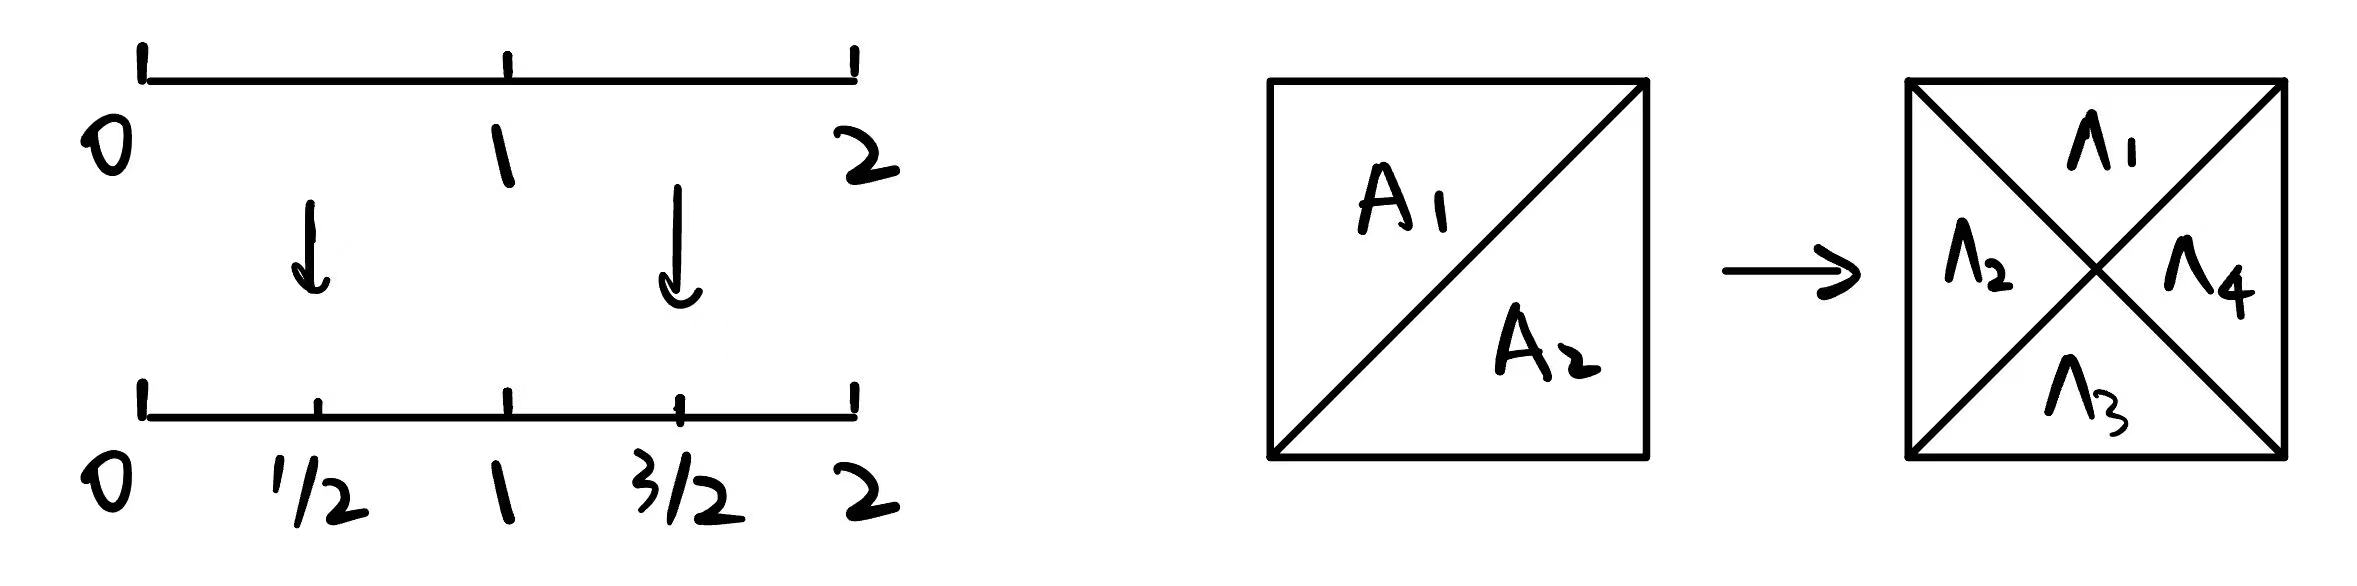
\includegraphics[width=0.8\textwidth]{figures/加细划分.jpg}
    \caption{加细划分}
\end{figure}

(Step 2) 对于 $\omega\in \Lambda_j,\forall j\geq 1$
\[
\begin{aligned}
    \EE(XY|\sigma(\Pi))(\omega) &= \EE(\sum_{k\geq 1}x_k\II_{\Lambda_k}Y|\sigma(\Pi))(\omega)\qquad [X=\sum_{k\geq 1}x_k\II_{\Lambda_k}]\\
    &=\EE(\sum_{k\geq 1}x_k\II_{\Lambda_k}Y|\Lambda_j)\qquad [\sigma(\Pi)\text{定义}]\\
    &=\EE(\sum_{k\geq 1}x_k\II_{\Lambda_k}Y\II_{\Lambda_j})/\PP(\Lambda_j)\qquad [\text{推论\eqref{cor:con_exp_indic}}]\\
    &=\EE(Yx_j\II_{\Lambda_j})/\PP(\Lambda_j)\qquad [\II_{\Lambda_k}\II_{\Lambda_j}\text{当}\Lambda_k\neq\Lambda_j\text{时}=0]\\
    &=x_j\EE(Y\II_{\Lambda_j})/\PP(\Lambda_j)\\
    &=x_j \EE(Y|\II_{\Lambda_j})\\
    &=X(\omega)\EE(Y|\II_{\Lambda_j})
\end{aligned}
\]

\[
\Rightarrow \EE(XY|\sigma(\Pi))=X\sum_{j\geq 1}\II_{\Lambda_j}\EE(Y|\Lambda_j)=X\EE(Y|\sigma(\Pi))
\]

数学上有种现象叫“法国人的伎俩”,即把定理当定义用。严格地讲,这么做有时会出现存在性和唯一性不满足的问题。下面介绍一个常被当做定义用的定理:

\begin{theorem}\label{thm:partition_con_exp}
    $\Pi=\{\Lambda_k,k\geq 1\}$ 为 $\Omega$ 的划分, $\EE|X|<\infty$。记 $Y:=\EE(X|\sigma(\Pi))=\sum_{k\geq 1}\II_{\Lambda_k}\EE(X|\Lambda_k)$,则
    \begin{enumerate}
        \item $Y$ 仍是一个离散随机变量,且 $\EE|Y|\geq \EE|X|<\infty$
        \item $\sigma(Y)\st \sigma(\Pi)$ (记作 $Y\in \sigma(\Pi)$,即 $Y$ 的所有信息都在 $\sigma(\Pi)$ 里)
        \item $\forall A\in \sigma(\Pi)$,有 $\EE(Y\II_A)=\EE(X\II_A)$
    \end{enumerate}
\end{theorem}

证明:(1)$E|X|=\sum_{x\in S_x}|x|\PP(X=x)<\infty$

\[
    \EE|Y|=\sum_{k\geq 1}|\EE(X|\Lambda_k)|\PP(\Lambda_k)\geq \sum_{k\geq 1}\sum_{x\in S}|x|\PP(\{X=x\}\cap \Lambda_k)
\]

逻辑上,现在第一个等号不成立,但之后 $<\infty$ 一写出来,之前的所有等号立刻成立,此处只为书写简便

\[
    \EE|X|=\sum_{x\in S_x}|x|\PP(X=x)=\sum_{x\in S}|x|\sum_{k\geq 1}\PP(\Lambda_k\cap \{X=x\})
\]

我们知道 $\sum_{x\in S}|x|\sum_{k\geq 1}\PP(\Lambda_k\cap \{X=x\})$ 绝对收敛,若求和次序交换后的 $\sum_{k\geq 1}\sum_{x\in S}|x|\PP(\{X=x\}\cap \Lambda_k)$ 也绝对收敛,则 $\EE|Y|<\infty$ 得证。有一个引理可以保证绝对收敛:

\begin{lemma}[\cite{calculus}.P280.推论]\label{lem:abs_convergence}
    从 273-280
\end{lemma}

\begin{corollary}[来自定理\ref{thm:partition_con_exp}(1)]\label{cor:double_exp}
    \begin{enumerate}
        \item (重期望公式)$\EE|\EE(X|\sigma(\Pi))|=\EE|X|, \EE(\EE(X|\sigma(\Pi)))=\EE(X)$
        \item $|\EE(X|\Lambda_k)|\leq \EE(|X|\mid\Lambda_k), |\EE(X|\sigma(\Pi))|\leq \EE(|X|\mid\sigma(\Pi))$
    \end{enumerate}
\end{corollary}

(2) 由定义,$Y=\sum_{k\geq 1}y_k\II_{\Lambda_k}$,其中 $y_k:=\EE(X|\Lambda_k)$

记 $S_Y=\cup_{k\geq 1}\{y_k\}$,注意到,可能 $\exists i\neq j$,但 $y_i=y_j$

故 $J_y=\{k|y_k=y\}(y\in S_Y)$ 中个数可能大于1

\[
Y=\sum_{y\in S_Y}y\II_{\sum_{k\in J_y}\Lambda_k}
\]

\[
\{Y=y\}=\sum_{k\in J_y}\Lambda_k\in \sigma(\Pi)
\]

\[
\sigma(Y)\st \sigma(\Pi)\qed
\]

(3) $\EE(Y\II_A)=\EE(\II_A\EE(X|\sigma(\Pi)))$

\[
\begin{aligned}
    \EE(Y\II_A)&=\EE(\II_A\EE(X|\sigma(\Pi)))\\
    &=\EE(\EE(X\II_A|\sigma(\Pi)))\qquad [A\in \sigma(\Pi), \text{性质\eqref{prt:extract_known}}]\\
    &=\EE(X\II_A)\qquad [\text{重期望-推论\eqref{cor:double_exp}}]
\end{aligned}
\]

\subsubsection*{$3^\circ$关于离散随机变量的条件期望}

\begin{definition}
    概率空间 $(\Omega,\CF,\PP)$,$X,Y$ 为离散随机变量,$\EE|X|<\infty$。定义 $\EE(X|Y)=\EE(X|\sigma(Y))=\EE(X|\sigma(\Pi_Y))$,称为 $X$ 关于 $Y$ 的条件期望
\end{definition}

注:$\omega=\{Y=y\}\in \Pi_Y$ 或 $Y(\omega)=y$,$\EE(X|Y)(\omega)=\EE(X|Y=y)$

\begin{example}
    $\EE(X|\Pi_{\Omega})=\EE(X|\sigma(\Omega))=\EE(X)$
\end{example}

\begin{example}
    $\II_A\ind \II_B\Rightarrow \EE(\II_A|\II_B)=[\text{Exa\eqref{exa:con_exp_indic}}]\EE(\II_A)$
\end{example}

\begin{example}
    $\EE(X|X)=\EE(X|\sigma(X))=X$[\text{Exa \ref{exa:extract_known}}]
\end{example}

\begin{property}
    假设以下期望、条件期望都有意义
    \begin{enumerate}
        \item $\EE(aX+bY|Z)=a\EE(X|Z)+b\EE(Y|Z)$
        \item $X\ind Y\Rightarrow \EE(X|Y)=\EE(X)$
        \item $\sigma(X)\st \sigma(Z)\Rightarrow \EE(XY|Z)=X\EE(Y|Z)$
        \item $\EE(\EE(X|Z))=\EE(X)$
        \item $|\EE(X|Z)|\leq \EE(|X|\mid Z)$
    \end{enumerate}
\end{property}

\subsubsection*{$4^\circ$关于多个离散随机变量的条件期望}

$\EE(Y|X_1,\cdots,X_n)$

\begin{enumerate}
    \item 由 $X_1,\cdots ,X_n$ 生成的 $\sigma$代数 $\sigma(X_1,\cdots,X_n)$
    \item $:=\EE(Y|\sigma(X_1,\cdots ,X_n))$
\end{enumerate}

怎样生成 $\sigma$代数可以包含 $X_1,\cdots,X_n$ 尽可能多的信息?

直觉是 $\bigcup_{k=1}^{\infty}\sigma(X_k)$,然而它不一定是 $\sigma$代数,因为它对可列并不封闭。

每个 \(\sigma(X_k)\) 是一个 \(\sigma\)代数,因此它对可列并封闭。

然而,\(\bigcup_{k=1}^{\infty} \sigma(X_k)\) 只是将每个 \(\sigma(X_k)\) 中的集合简单地并在一起,并没有保证这些集合的可列并仍然在 \(\bigcup_{k=1}^{\infty} \sigma(X_k)\) 中。

例如,假设 \(X_k \in \sigma(X_k)\),那么 \(X_k\) 在 \(\bigcup_{k=1}^{\infty} \sigma(X_k)\) 中,但 \(\bigcup_{k=1}^{\infty} X_k\) 可能不在 \(\bigcup_{k=1}^{\infty} \sigma(X_k)\) 中,因为它可能不属于任何一个单独的 \(\sigma(X_k)\)。问题出在 \(\bigcup_{k=1}^{\infty} \sigma(X_k)\) 缺少 $\{\sigma(X_k)\}_{k\geq 1}$ 交互的部分

怎样把 \(\bigcup_{k=1}^{\infty} \sigma(X_k)\) 变成$\sigma$代数?

\begin{definition}[多个离散随机变量的条件期望]\label{def:multi_rv_con_exp}
    定义由离散随机变量 $X_1,\cdots,X_n$ 生成的 $\sigma$代数
    \[
    \begin{aligned}
        \sigma(X_1,\cdots,X_n)&:=(X_1,\cdots,X_n)^{-1}(2^{S_1}\times \cdots \times 2^{S_n})\\
        &:=\{\underbrace{(X_1,\cdots,X_n)^{-1}(A_1\times\cdots\times A_n)}_{\text{柱集}}|A_1\times\cdots\times A_n\st \underbrace{S_1\times\cdots\times S_n}_{\text{乘积空间}}\}\\
        &=\{\bigcap_{k=1}^{\infty}X_k^{-1}(A_k)|A_k\in 2^{S_k},1\leq k\leq n\}
    \end{aligned}
    \]
\end{definition}

\begin{theorem}\label{thm:discrete_rv_partition}
    令 $x_k=\sum_{i\geq 1}x_{k,i}\II_{\Lambda_{k,i}}, 1\leq k\leq n$,为离散随机变量,对每一个 $k$,$\Pi_k:=\{\Lambda_{k,i}|i\geq 1\}$ 为 $\Omega$ 的划分,定义
    \[
    \Pi_{(X_1,\cdots,X_n)}:=\{\Lambda_{1,i_1}\cap\cdots \cap \Lambda_{n,i_n}|i_k\geq 1,1\leq k\leq n\}
    \]
    则
    \begin{enumerate}
        \item $\Pi_{(X_1,\cdots,X_n)}$ 是 $\Omega$ 的划分,且
        \[
            \sigma(\Pi_{(X_1,cdots,X_n)})=\left \{\sum_{\substack{(i_1,\cdots ,i_n) \\ \in J_1\times \cdots \times J_n}} (\Lambda_{1,i_1}\cap \cdots \cap \Lambda_{1,i_n})|J_k\st \NN,1\leq k\leq n\right \}
        \]
        \item $\sigma(X_1,\cdots,X_n)=\sigma(\Pi_{(X_1,\cdots ,X_n)})$(即定义\ref{def:multi_rv_con_exp}是有意义的,well-defined,make sense,良定义)
    \end{enumerate}
\end{theorem}

\begin{problem}[作业2-2]
    证明定理\ref{thm:discrete_rv_partition}在 $n=2$ 时成立
\end{problem}

\begin{definition}
    $\EE|Z|<\infty$ 定义
    \[
    \EE(Z|X_1,\cdots,X_n)=\EE(Z|\sigma(X_1,\cdots,X_n)):=\EE(Z|\sigma(\Pi_{(X_1,\cdots,X_n)}))
    \]
\end{definition}

\begin{definition}\label{def:multi_rv_indep}
    $(\Omega,\CF,\PP), Y:\Omega\to S_Y, X_1:\Omega\to S_1,X_2:\Omega\to S_2$ 为离散随机变量,称 $Y$ 和 $(X_1,X_2)$ 独立,若 $\sigma(Y)\ind \sigma(X_1,X_2)$. [$\sigma(Y)=Y^{-1}(2^{S_Y}),\sigma(X_1,X_2)=(X_1,X_2)^{-1}(2^{S_1}\times 2^{S_2})$]

    即 $\forall A\st S_Y,B\st 2^{S_1}\times 2^{S_2}, B=B_1\times B_2$,有 
    \[
    \PP(Y\in A,(X_1,X_2)\in B)=\PP(Y\in A)\PP((X_1,X_2)\in B)
    \]
    其中 $\PP((X_1,X_2)\in B)=\PP(X_1\in B_1,X_2\in B_2)$
\end{definition}

\begin{problem}[作业2-3]
    证明:
    \[
    \begin{aligned}
        Y\ind (X_1,X_2)\Leftrightarrow &\forall y\in S_Y,x_1\in S_1,x_2\in S_2\\
        &\text{有}\PP(Y=y,(X_1,X_2)=(x_1,x_2))\\
        &=\PP(Y=y)\PP((X_1,X_2)=(x_1,x_2))
    \end{aligned}
    \]
\end{problem}

有了上述定义,可以推广:

\begin{enumerate}
    \item $(Y_1,\cdots,Y_n)\ind (X_1,\cdots,X_n)$
    \item $Y\ind_A (X_1,\cdots,X_n) (A\in \CF,\PP(A)>0)$
\end{enumerate}

\begin{property}\label{prop:pairwise_indep}
    $Y\ind (X_1,X_2)\Rightarrow Y\ind X_1,Y\ind X_2$
\end{property}

证明:在定义\ref{def:multi_rv_indep}中取$B_2=\Omega$

\[
\begin{aligned}
    \PP(Y\in A,X_1\in B_1)&=\PP(Y\in A,X_1\in B_1,X_2\in S_2)\\
    &=\PP(Y\in A)\PP(X_1\in B_1,X_2\in S_2)\qquad [Y\ind (X_1,X_2)]\\
    &=\PP(Y\in A)\PP(X_1\in B_1)
\end{aligned}
\]

注:看到 $\Rightarrow$ 要自然地问,反过来 $\Leftarrow$ 成立吗?做数学要多问自己一些问题,即便没有答案

\begin{corollary}
    $(Y_1,\cdots,Y_n)\ind (X_1,\cdots,X_n)\Rightarrow Y_k\ind X_j, 1\leq k\leq m,1\leq j\leq n$
\end{corollary}

\subsection{随机过程}

\subsubsection{什么是随机过程}

\begin{definition}[随机过程]
    设 $(\Omega, \CF, \PP)$ 为概率空间,$(S,\CS)$ 为可测空间,$\TT$ 为指标集/参数集,称随机变量族
    \[
    \{X_t: (\Omega,\CF,\PP)\rightarrow (S,\CS)|t\in \TT\}
    \]
    为 (S值) 随机过程 $X$。其中 $(S,\CS)$ 称为 $X$ 的状态空间

    注:\begin{enumerate}
        \item $forall t\in \TT$,$X_t$ 为随机变量
        \item $\TT$ 为时间集,$X_t$ 为过程 $X$ 在时刻 $t$ 的状态
    \end{enumerate}
\end{definition}

\[
\begin{array}{c|cc}
    \TT \backslash S \st \RR & \text{离散 }(e.g.\ \NN) & \text{连续 }(e.g.\ \RR,\RR^+) \\ \hline
    \text{可数集 }(e.g.\ \NN,\ZZ) & \multicolumn{2}{c}{\text{离散时间/参数的随机过程}} \\
    \text{连续统 }(e.g.\ [0,T],\RR^+) & \multicolumn{2}{c}{\text{连续时间/参数的随机过程}}
\end{array}
\]

\subsubsection{随机过程的分布}

\begin{enumerate}
    \item $\forall t\in \TT, X_t:\Omega\rightarrow S$ 为随机变量/可测映射
    \item $X: \TT\times \Omega\rightarrow S$ 二元映射
    \item $X:\Omega\rightarrow S^{\TT}$ 其中 $S^{\TT}=\{f|f:\TT\rightarrow \S\}$,$X:\omega\rightarrow X(\omega)=X(\cdot,\omega)$
\end{enumerate}

分布可用有限维分布族刻画

\begin{definition}
    固定样本点 $\omega$,则 $X_{\cdot}(\omega)$ 为 $\TT\rightarrow S$ 的映射,即 $X_{\cdot}(\omega)\in S^{\TT}$,称 $X_{\cdot}(\omega)$ 是过程 $X$ 的一个实现/样本路径/样本函数
\end{definition}

\begin{definition}
    $\forall n\geq 1, t_1,t_2,\cdots,t_n$ 称 
    \[
    (x_1,x_2,\cdots,x_n)\mapsto F_{t_1,t_2,\cdots,t_n}(x_1,x_2,\cdots,x_n)=\PP(X_{t_1}\leq x_1,\cdots, X_{t_n}\leq x_n)
    \]
    为 $X$ 的 $n$ 维分布
\end{definition}

\begin{definition}[过程的有限维分布族]
    定义
    \[
    \{F_{t_1,t_2,\cdots,t_n}|n\geq 1,t_1,\cdots,t_n\in \TT\}
    \]
\end{definition}

\subsubsection{随机过程的存在性}

\begin{enumerate}
    \item (抽象的) 从概率论/测度论出发去证明随机过程存在性,不写出具体形式,满足随机过程符合给定的有限维分布族即可
    \item (具体的) 构造性证明
\end{enumerate}

\begin{property}
随机过程的有限维分布族具有以下两个性质
\begin{enumerate}
    \item (对称性) 重排,设 $\sigma:\{1,\cdots,n\}\rightarrow \{1,\cdots,n\}$ 为双射,则
    \[
    F_{t_{\sigma(1)}, \cdots,t_{\sigma(n)}}(x_{\sigma(1)},\cdots,x_{\sigma(n)})=F_{t_1,\cdots,t_n}(x_1,\cdots,x_n)
    \]
    \item (相容性) $m\geq n$
    \[
    F_{t_1,\cdots,t_n,t_{n+1},\cdots,t_m}(x_1,\cdots,x_n,+\infty,\cdots,+\infty)=F_{t_1,\cdots,t_n}(x_1,\cdots,x_n)
    \]
    注:相容性类比从高维向低维的投影,$\PP(X\leq +\infty)=F_X(+\infty)=1$
\end{enumerate}
这两个性质是随机过程存在的必要条件
\end{property}

\begin{theorem}[Kolmogorov定理]\label{thm:Kolmogorov}
    设分布函数族
    \[
    \{F_{t_1,\cdots,t_n}|t_1,\cdots,t_n\in \TT,n\geq 1\}
    \]
    满足\uwave{对称性},\uwave{相容性},则必存在一个随机过程 $\{X_t,t\in \TT\}$ 使得上述分布函数族 $F$ 是 $X$ 的有限维分布族
\end{theorem}

\subsubsection{随机过程的基本类型}

\begin{enumerate}
    \item 离散时间马氏链(由条件概率定义)
    \item Poisson 过程
    \item 更新过程
    \item 连续时间马氏链
    \item 离散时间 Martingale (由条件期望定义)
    \item 布朗运动
\end{enumerate}

\begin{definition}
    对连续时间的随机过程 $\{X_t,t\in \TT\}$
    \begin{enumerate}
        \item 若对一切的 $t_0<t_1<\cdots<t_n$ 有 $X_{t_1}-X_{t_0},\cdots,X_{t_n}-X_{t_{n-1}}$ 相互独立,则过程 $X$ 是独立增量过程(e.g. 布朗运动)
        \item 若对每一个 $S\in \TT, X_{t+s}-X_t$ 对一切的 $t$ 都有相同分布,称 $X$ 为平稳增量过程
    \end{enumerate}
\end{definition}

\pagebreak

\section{马氏链}
\subsection{离散时间马氏链}

马尔可夫性 $\leftrightarrow$ 已知现在,过去与未来不相干/独立

\begin{definition}[(离散时间)马氏链]\label{def:M_1}
    称 $S$ 值随机过程 $\{X_n,n\geq 0\}$ 为马氏链,若 $X$ 满足以下马氏性:$\forall n\geq 0,x_0,x_1,\cdots,x_n,y\in S$,
    \[
    \PP(\underbrace{X_{n+1}=y}_{\text{未来}}|\underbrace{X_0=x_0,\cdots,X_{n-1}=x_{n-1}}_{\text{过去}},\underbrace{X_n=x_n}_{\text{现在}})=\PP(X_{n+1}=y|X_n=x_n)\label{eq:M1}\tag{$M_1$}
    \]
    其中 $X_0$ 的分布称为 $X$ 的初始分布
\end{definition}

\begin{definition}
    当 $S$ 为有限集,称链为有限链,当 $S$ 为无限集,称链为无限链
\end{definition}

注:改写 $(M_1)$
\[
LHS=\PP_{X_n=x_n}(X_{n+1}=y|X_0=x_0,\cdots,X_{n-1}=x_{n-1})
\]
\[
RHS=\PP_{X_n=x_n}(X_{n+1}=y)
\]
\[
\begin{aligned}
    M_1 &\Leftrightarrow \{X_{n+1}=y\}\ind_{\{X_n=x_n\}}\{X_0=x_0,\cdots,X_{n-1}=x_{n-1}\}\\
    &\Leftrightarrow X_{n+1}\ind_{\{X_n=x_n\}} (X_0,\cdots,X_{n-1})
\end{aligned}
\]
$(M_1)\quad \text{未来}\ind_{\text{现在}}\text{过去}$
\[
\PP_{\text{现在}}(\text{未来}|\text{过去})=\PP_{\text{现在}}(\text{未来})
\]

\begin{lemma}[马氏性的等价表示]\label{lem:markov_equiv}
    [Grimmett\cite{grimmett}] 下面三个命题等价
    \begin{enumerate}
        \item $(M_1)$ 马氏性
        \item $\forall k\geq 0, 0\leq n_1< \cdots<n_k\leq n$,对于 $y,x_{n_1},\cdots,x_{n_k}\in S$,
        \[
        \PP(X_{n+1}=y|X_{n_1}=x_{n_1},\cdots,X_{n_k}=x_{n_k})=\PP(X_{n+1}=y|X_{n_k}=x_{n_k})\tag{$M_2$}
        \]
        即
        \[
        \{X_{n+1}=y \}\ind_{\{X_{n_k}=x_{n_k}\}}\{X_{n_1}=x_{n_1},\cdots,X_{n_{k-1}}=x_{n_{k-1}}\}
        \]
        \item 对 $\forall m\geq 1,n\geq 0, \{y,x_i,0\leq i\leq n\}\st S$,有
        \[
        \PP(X_{n+m}=y|X_0=x_0,\cdots,X_n=x_n)=\PP(X_{n+m}=y|X_n=x_n)\tag{$M_3$}
        \]
        即
        \[
        \{X_{n+m}=y\}\ind_{\{X_n=x_n\}}\{X_0=x_0,\cdots,X_{n-1}=x_{n-1}\}
        \]
    \end{enumerate}
\end{lemma}

证明:思路 $1\leftrightarrows 3\leftrightarrows 2$

$(2)\rightarrow (3)$,先处理一些记号的问题。记(2)中的 $n$ 为 $n^{(2)}$, (3)中的 $n$ 为 $n^{(3)}$。则取 $n_k=n^{(3)}=n^{(2)}+1-m\leq n^{(2)}$,所以 $n^{(3)}+m=(n^{(2)}+1-m)+m=n^{(2)}+1$,即已知(2)可推(3)

$(3)\rightarrow (1)$,取 $m=1$,显然

只需证 $(3)\rightarrow (2),(1)\rightarrow (3)$

这里回顾独立的三种写法
\begin{enumerate}
    \item $A\ind_B C$ 记号
    \item $\PP_B(A,C)=\PP_B(A)\PP_B(C)$ 定义
    \item $\PP_B(A|C)=\PP_B(A)$ 定理
\end{enumerate}

(Step 1) 证明 $(3)\rightarrow (2)$

思路:(2)(3)条件不同,想要由(3)推(2),则切换到(2)的条件概率测度,展开,再用(3)的条件瘦身

对 $\forall k\geq 2, 0\leq n_1<n_2<\cdots<n_k=n$

令 $J=\{0,1,\cdots,n_k-1,n_k\}\backslash \{n_1,\cdots,n_k\}$, $\tilde{\PP}(\cdot)=\PP(\cdot|X_{n_1}=x_{n_1},\cdots,X_{n_k}=x_{n_k})$

\[
\begin{aligned}
    \tilde{\PP}(X_{n+1}=y)&=\sum_{x_j\in S,j\in J}\tilde{\PP}(X_{n+1}=y|X_j=x_j,j\in J)\cdot\tilde{\PP}(X_j=x_j,j\in J)\qquad [\text{全概公式}]\\
    &=\PP(X_{n+1}=y|X_{n_k}=x_{n_k})\sum_{x_j\in S,j\in J}\tilde{\PP}(X_j=x_j,j\in J)\qquad [(3), \PP_C(\cdot|A)=\PP_C(\cdot)]\\
    &=\PP(X_{n+1}=y|X_{n_k}=x_{n_k})
\end{aligned}
\]

其中,记号 $\sum_{x_j\in S,j\in J}$ 中的下标意为:假设 $J$ 中元素个数为 $\# J=u$,则 $(x^{(1)},\cdots, x^{(u)})\in S^u$。从简单的开始,$\sum_{x\in S}\PP(X=x)=\PP(\Omega), \sum_{(x,y)\in S^2}\PP(X=x,Y=y)=\PP(\Omega),\cdots$,$\sum_{(x^{(1)},\cdots, x^{(u)})\in S^u}\PP(X^{(1)}=x^{(1)},\cdots,X^{(u)}=x^{(u)})=\PP(\Omega)=1$

(Step 2) 下证 $(1)\rightarrow (3)$

1. $m=1$ 时,即 $(1)$

2. 假设 $m=k$ 时 $(3)$ 成立,即 $\forall n\geq 1, \{y,x_i,n\geq i\geq 0\}\st S$,
\[
\{X_{n+k}=y\}\ind_{\{X_n=x_n\}}\{X_0=x_0,\cdots, X_{n-1}=x_{n-1}\}\xrightarrow{\text{性质\eqref{prop:pairwise_indep}}}\{X_{n+k}=y\}\ind_{\{X_n=x_n\}}\{X_{n-1}=x_{n-1}\}
\]
\[
\begin{aligned}
    \PP(X_{n+k}=y|X_0=x_0,\cdots,X_n=x_n)&=\PP(X_{n+k}=y|X_n=x_n)\\
    &=\PP(X_{n+k}=y|X_n=x_n,X_{n-1}=x_{n-1})
\end{aligned}\tag{*}
\]
当 $m=k+1$ 时,对 $\forall \{y,x_i,n\geq i\geq 0\}\st S$

令 $\tilde{\PP}_n(\cdot):=\PP(\cdot|X_0=x_0,\cdots,X_n=x_n)$
\[
\begin{aligned}
    \tilde{\PP}_n(X_{n+k+1}=y)&=\sum_{x_{n+1}\in S}\tilde{\PP}_n(X_{n+k+1}=y|X_{n+1}=x_{n+1})\cdot \tilde{\PP}_n(X_{n+1}=x_{n+1})\quad [\text{定理}\eqref{thm:law_total_prob}]\\
    &=\sum_{x_{n+1}\in S}\PP(X_{n+k+1}=y|X_{n+1}=x_{n+1},X_n=x_n)\cdot \PP(X_{n+1}=x_{n+1}|X_n=x_n)\quad [\text{(*), 归纳法假设}]\\
    &=\sum_{x_{n+1}\in S}\PP(X_{n+k+1}=y,X_{n+1}=x_{n+1},X_n=x_n)/\PP(X_n=x_n)\quad [\text{乘法公式\eqref{eq:multiply_func}}]\\
    &=\PP(X_{n+k+1}=y,X_n=x_n)/\PP(X_n=x_n)\\
    &=\PP(X_{n+k+1}=y|X_n=x_n)
\end{aligned}
\]
即 $m=k+1$ 得证\qed

证明 (Step 2) 时如果在 $x_{n+k}$ 处展开而不是在 $x_{n+1}$,也是可以的。实际上在 $x_{n+j}, \forall j, 1\leq j\leq k$ 展开都可以,关键在于用性质\ref{prop:pairwise_indep}和全概公式\ref{thm:law_total_prob}凑出乘法公式\eqref{eq:multiply_func},消元即可。

\begin{remark}
    三种写法的直觉
    \begin{enumerate}
        \item $M_1$:未来“下一步”跟过去“每一步”都无关
        \item $M_2$:未来“下一步”跟过去的“任意若干步”都无关
        \item $M_3$:未来“下m步”跟过去“每一步”都无关
    \end{enumerate}
    可以推出,由(2)(3),下式也成立:
    
    对 $\forall m\geq 1,n\geq 0, \{y,x_i,0\leq i\leq n\}\st S$
    \[
    \PP(X_{n+m}=y|X_{n_1}=x_{n_1},\cdots,X_{n_k}=x_{n_k})=\PP(X_{n+m}=y|X_{n_k}=x_{n_k})
    \]
\end{remark}

\begin{corollary}\label{cor:markov_con_cut}
    若 $X$ 是马氏链,则 $\forall n\geq 1,\{x_i,n\geq i\geq 0,y\}\st S$,有 
    \[
    \PP(X_{n+1}=y|X_0=x_0,\cdots,X_n=x_n)=\PP(X_{n+1}=y|X_n=x_n,X_{n-1}=x_{n-1})
    \]
\end{corollary}

补充记号:
\begin{itemize}
    \item 乘积空间
    \[
        S^n:=\underbrace{S\times\cdots\times S}_{\text{n个}}
    \]
    \item 乘积 $\sigma$ 代数
    \[
        \bigotimes_n 2^S:=\underbrace{2^S\times\cdots\times 2^S}_{\text{n个}}
    \]
\end{itemize}

\begin{property}[马氏性的等价条件]\label{prt:markov_equiv_condition}
下列三个命题等价
\begin{enumerate}
    \item 马氏性 $(M_1)$
    \item 对 $\forall n\geq 1,m\geq 1,A\in \otimes_n 2^S,B\in \otimes_m 2^S$,即 $(A\st S^n,B\st S^m)$,有
    \begin{equation}
    \begin{aligned}
        &\PN((X_0,\cdots,X_{n-1})\in A,(X_{n+1},\cdots,X_{n+m})\in B)\\
        =&\PN((X_0,\cdots,X_{n-1})\in A)\cdot \PN((X_{n+1},\cdots,X_{n+m})\in B)
    \end{aligned}
    \label{eq:markov_equiv_condition_M2}
    \end{equation}
    即 $(X_0,\cdots,X_{n-1})\ind_{\{X_n=x_n\}}(X_{n+1},\cdots,X_{n+m})$ 的定义
    \item $\PN((X_{n+1},\cdots,X_{n+m})\in B|(X_0,\cdots,X_{n-1})\in A)=\PN((X_{n+1},\cdots,X_{n+m})\in B)$
\end{enumerate}
\end{property}

证明:$(2)\Leftrightarrow (3)$,独立的定义和定理,显然

$(3)\rightarrow (1)$,取 $k=0$ 显然

只需证 $(1)\rightarrow (3)$

只需证 $(3)$ 对简单事件 $A,B$ (单点集合) 成立,即 $\forall n\geq 1,m\geq 1, \{x_0,x_1,\cdots,x_{n+m}\st S\}$,有
\[
\PN((X_{n+1},\cdots,X_{n+m})=x_{n+1}^{n+m}|(X_0,\cdots,X_{n-1})=x_0^{n-1})=\PN((X_{n+1},\cdots,X_{n+m})=x_{n+1}^{n+m})
\]
其中 $x_{n+1}^{n+m}=(x_{n+1},\cdots,x_{n+m}),x_{0}^{n-1}=(x_0,\cdots,x_{n-1})$

*只要对单点集合成立,对一般情况也成立,证明见定理\ref{thm:independent_rv}

只证 $m=2$,令
\[
\tilde{\PP}_n(\cdot):=\PN(\cdot|(X_0,\cdots,X_{n-1})=x_0^{n-1})=\PP(\cdot|(X_0,\cdots,X_{n})=x_0^{n})
\]
$\Rightarrow$
\[
\begin{aligned}
    \tilde{\PP}_n((X_{n+1},X_{n+2})=(x_{n+1},x_{n+2}))&=\tilde{\PP}_n(X_{n+1}=x_{n+1})\cdot \tilde{\PP}_n(X_{n+2}=x_{n+2}|X_{n+1}=x_{n+1})\\
    &=\PP(X_{n+1}=x_{n+1}|X_n=x_n)\cdot \PP(X_{n+2}=x_{n+2}|X_{n+1}=x_{n+1})\qquad [M_1]\\
    &=\PP(X_{n+1}=x_{n+1}|X_n=x_n)\cdot \PP(X_{n+2}=x_{n+2}|X_{n+1}=x_{n+1},X_n=x_n)\qquad [\text{推论\eqref{cor:markov_con_cut}}]\\
    &=\PN(X_{n+1}=x_{n+1})\cdot \PN(X_{n+2}=x_{n+2}|X_{n+1}=x_{n+1})\\
    &=\PN((X_{n+1},X_{n+2})=(x_{n+1},x_{n+2}))\qquad [\text{乘法公式\eqref{eq:multiply_func}}]
\end{aligned}
\]

\begin{corollary}
    设 $X$ 为马氏链,则对每一个 $n\geq 1,m\geq 1, u_k<u_{k+1}, 0\leq k\leq n+m-1$,有
    \[
    (X_{u_0},\cdots,X_{u_{n-1}})\ind_{\{X_{u_n}=x_{u_n}\}}(X_{u_{n+1}},\cdots,X_{u_{n+m}})
    \]
\end{corollary}

\subsection{时齐马氏链与转移概率}

\begin{definition}[时间齐次马氏链]
    称马氏链 $X:\{X_n,n\geq 0\}$ 为时齐的或时间齐次马氏链,若对 $\forall n\geq 0, i,j\in S$
    \[
    \PP(X_{n+1}=j|X_n=i)=\PP(X_1=j|X_0=i)
    \]
\end{definition}

\begin{definition}
    $X$ 是时齐马氏链,称
    \[
    p_{ij}:=p_{i,j}=\PP(X_1=j|X_0=i)\qquad i,j\in S
    \]
    为 $X$ 从状态 $i$ 到 $j$ 的(一步)\textbf{转移概率},并称矩阵
    \[
    P=\begin{bmatrix}
        p_{11} & p_{12} & p_{13} & \cdots\\
        p_{21} & p_{22} & p_{23} & \cdots\\
        \vdots & \vdots & \vdots & \ddots
    \end{bmatrix}
    \]
    为(一步)转移(概率)矩阵
\end{definition}

若不加说明,则默认讨论的马氏链都是时齐的

注:
\[
\begin{aligned}
    \PP(x_{n+1}=y)&=\sum_{x\in S}\PP(X_{n+1}=y|X_n=x)\cdot \PP(X_n=x)\\
    &=\sum_{x\in S}p_{xy}\cdot \PP(X_n=x)
\end{aligned}
\]

\begin{theorem}[转移矩阵的刻画]\label{thm:random_matrix}
    转移矩阵是一个随机矩阵,即
    \begin{enumerate}
        \item $\forall i,j\in S,p_{ij}\geq 0$
        \item $\forall i\in S,\sum_{j\in S}p_{ij}=1$
    \end{enumerate}
    即转移矩阵的每一行 $(p_{ij})_{j\in S}$ 为 $S$ 上的一个概率分布

    注:另一种随机矩阵是指元素为随机变量的矩阵,和这里讲的没有关系
\end{theorem}

证明:
\[
\sum_{j\in S}\PP(X_1=j|X_0=i)=\PP(X_1\in S|X_0=i)=\PP(\Omega|X_0=i)=1
\]

\begin{definition}[时齐马氏链]\label{def:homo-markov}
    设 $X=\{X_n,n\geq 0\}$ 为一随机过程,若
    \begin{enumerate}
        \item 初值 $X_0$ 满足分布 $\mu=(\mu_i)_{i\in S}$,即 $\PP(X_0=i)=\mu_i,i\in S$
        \item 存在一个随机矩阵 $P=(p_{ij})_{i,j\in S}$ 使得 $\forall n\geq 1,i_0,\cdots,i_{n-1},i,j\in S$
        \[
        \PP(X_{n+1}=j|X_0=i_0,\cdots,X_{n-1}=i_{n-1},X_n=i)=p_{ij}
        \]
    \end{enumerate}
    则称 $X$ 具有初始分布 $\mu$ 和转移矩阵 $P$ 的(时齐)马氏链,记作 $X\sim \text{Markov}(\mu,P)$
\end{definition}

上述定义与$(M_1)$马氏链定义\ref{def:M_1}等价

证明:$(2)\rightarrow (M_1)$
\[
\begin{aligned}
    \PP(X_{n+1}=j|X_n=i)&=\sum_{(i_0,\cdots,i_{n-1})\in S^n}\PP(X_{n+1}=j|X_n=i,X_0=i_0,\cdots,X_{n-1}=i_{n-1})\PP(X_0=i_0,\cdots,X_{n-1}=i_{n-1})\\
    &=\sum_{(i_0,\cdots,i_{n-1})\in S^n}p_{ij}\cdot \PP(X_0=i_0,\cdots,X_{n-1}=i_{n-1})=p_{ij}
\end{aligned}
\]
所以 $\PP(X_{n+1}=j|X_0=i_0,\cdots,X_{n-1}=i_{n-1},X_n=i)=\PP(X_{n+1}=j|X_n=i)$

即然有 $(M_1)$,为什么还要定义\ref{def:homo-markov}?因为该定义决定了马氏链的有限维分布

\begin{example}[Gambler's Ruin]
    [Durrett\cite{durrett},P1] 
    \begin{figure}[H]
        \centering
        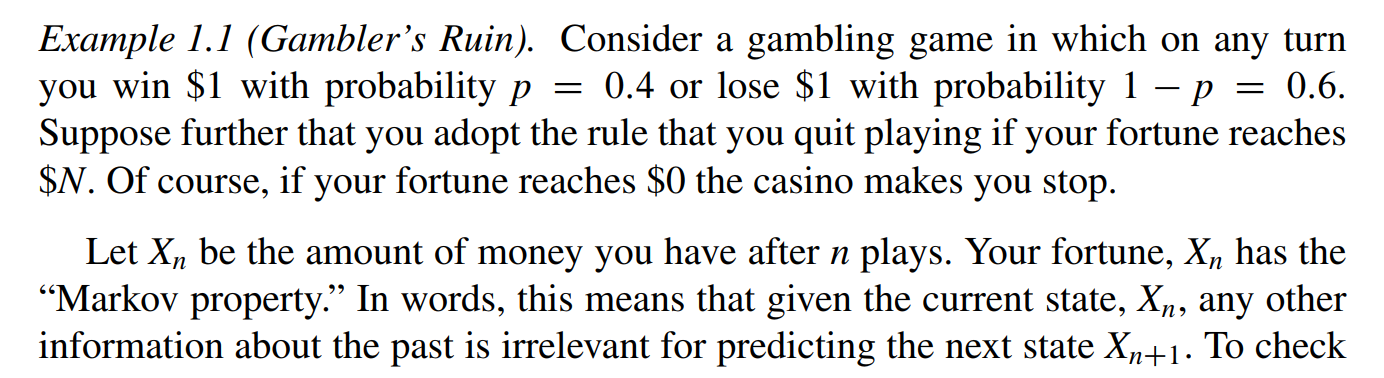
\includegraphics[width=0.9\textwidth]{figures/Gambler's Ruin.png}
        \caption{Gambler's Ruin}
    \end{figure}
\end{example}

\begin{claim}
$\{X_n,n\geq 0\}$ 为(时齐)马氏链
\end{claim}

1. 对于 $0<i_0,\cdots,i_{n-1}<N, n\geq 0$ 有
\[
\begin{aligned}
    &\PP(X_{n+1}=i+1|X_n=i,X_0=i_0,\cdots,X_{n-1}=i_{n-1})\\
    =&\PP(X_{n+1}=i+1|X_n=i)=0.4=\PP(\text{第}n+1\text{次赌局赢一元})
\end{aligned}
\]
\[
\begin{aligned}
    &\PP(X_{n+1}=i-1|X_n=i,X_0=i_0,\cdots,X_{n-1}=i_{n-1})\\
    =&\PP(X_{n+1}=i-1|X_n=i)=0.6=\PP(\text{第}n+1\text{次赌局输一元})
\end{aligned}
\]

2. $\PP(X_{n+1}=0|X_n=0,X_0=i_0,\cdots,X_{n-1}=i_{n-1})=1=\PP(X_{n+1}=0|X_n=0)$

$\PP(X_{n+1}=N|X_n=N, X_0=i_0,\cdots, X_{n-1}=i_{n-1})=1=\PP(X_{n+1}=N|X_n=N)$

最后一个等号是由题目设定得到,从 $0\to 0$ 或 $N\to N$ 的概率都为1,因为游戏结束

综上,$p(i,i+1)=0.4,0<i<N, p(i,i-1)=0.6, 0<i<N, p(0,0)=p(N,N)=1$

e.g. 

\begin{figure}[H]
    \centering
    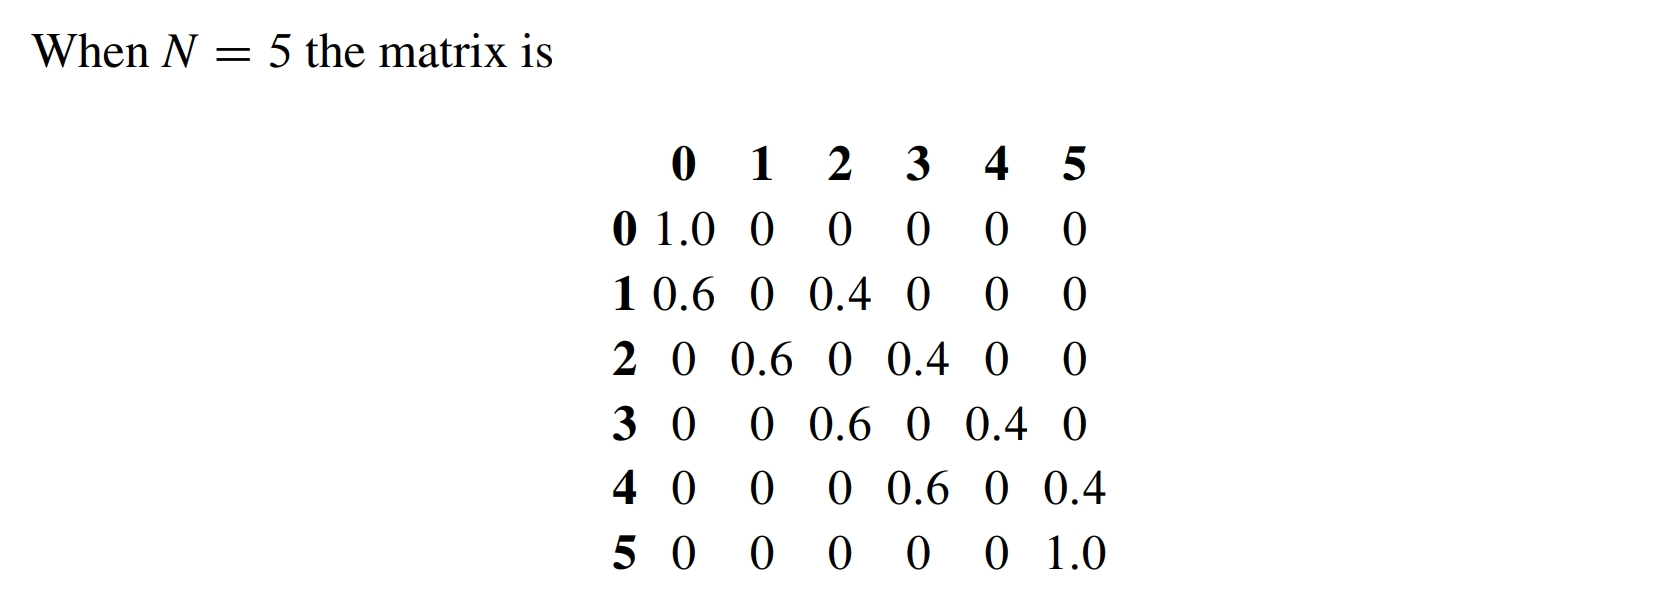
\includegraphics[width=0.9\textwidth]{figures/N=5.png}
    \caption{N=5}
\end{figure}

\begin{example}[Two-Stage Markov Chains]
    [Durrett\cite{durrett}, P7]
    \begin{figure}[H]
        \centering
        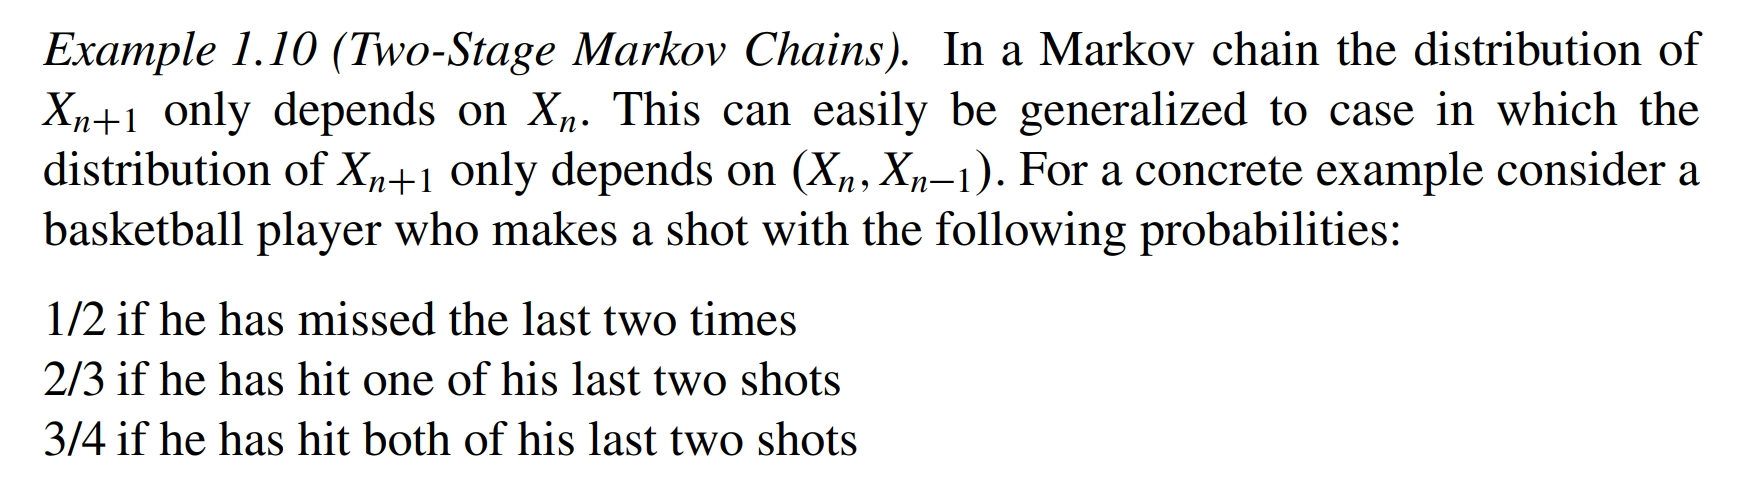
\includegraphics[width=0.9\textwidth]{figures/two_stage_markov_chains.png}
        \caption{Two-Stage Markov Chains}
    \end{figure}
\end{example}

\begin{enumerate}
    \item $\PP(X_{n+1}=H|X_n=M,X_{n-1}=M)=1/2$
    \item $\PP(X_{n+1}=H|X_n=M,X_{n-1}=H)=\PP(X_{n+1}=H|X_n=H,X_{n-1}=M)=2/3$
    \item $\PP(X_{n+1}=H|X_n=H,X_{n-1}=H)=3/4$
\end{enumerate}

\begin{claim}
$Y_n=(X_n,X_{n-1}), n\geq 1$ 则 $\{Y_n,n\geq 1\}$ 是(时齐)马氏链,$Y_n:\Omega\to \{HH,HM,MH,MM\}$ 
\end{claim}

证明:
\[
\begin{aligned}
    &\PP(Y_{n+1}=HH|Y_n=HH,Y_j=(x_j,x_{j-1}), 1\leq j\leq n-1)\\
    =& \PP(X_{n+1}=H,X_n=H|X_n=H,X_{n-1}=H,X_j=x_j,X_{j-1}=x_{j-1},0\leq j\leq n-1)\\
    =& \PP(X_{n+1}=H|X_n=H,X_{n-1}=H)\\
    =&3/4\qquad [3.]
\end{aligned}
\]

对 1.2. 同理\qed

\begin{proposition}[初见马氏链的有限维分布]\label{prop:markov_dist}
设 \(P = (p_{ij})_{i,j \in S}\) 为随机矩阵,\(\mu = (\mu_i)_{i \in S}\) 为概率分布,\(X = \{X_n, n \geq 0\}\) 为 \(S\) 值离散时间随机过程。则过程 \(X \sim \text{Markov}(\mu, P)\) 当且仅当对任意的 \(n \geq 0, i_0, i_1, \cdots, i_n \in S\),\(X\) 有有限维分布:
\begin{equation}
P(X_0 = i_0, X_1 = i_1, \cdots, X_n = i_n) = \mu_{i_0} \prod_{k=0}^{n-1} p_{i_k i_{k+1}}
\label{eq:markov_dist}
\end{equation}

\end{proposition}

证明:$\Rightarrow$ 
\[
\begin{aligned}
    &\PP(X_0=i_0,X_1=i_1,\cdots,X_n=i_n)\\
    =&\PP(X_0=i_0)\PP(X_1=i_1|X_0=i_0)\cdots \PP(X_n=i_n|X_0=i_0,\cdots X_{n-1}=i_{n-1})\quad [\text{乘法公式}\eqref{eq:multiply_func}]\\
    =&\PP(X_0=i_0)\PP(X_1=i_1|X_0=i_0)\cdots \PP(X_n=i_n|X_{n-1}=i_{n-1})\quad [\text{Markov}]\\
    =&\mu_{i_0}P_{i_0,i_1}\cdots P_{i_{n-1},i_n}
\end{aligned}
\]
严格地讲,$\PP(\cdot|A)$ 需保证 $\PP(A)>0$。对 $\PP(A)=0$ 情况的分类讨论,见 Resnick\cite{resnick}, prop 2.1.1 (\href{https://dafuzhuu.github.io/stochastic-process/pdf/Resnick.pdf}{PDF链接})

$\Leftarrow$ 

1. $n=0, \PP(X_0=i_0)=\mu_{i_0}\Rightarrow X_0\sim (\mu_i)_{i\in S}$

2. 
\[
\PP(X_{n+1}=i_{n+1}|X_0=i_0,\cdots,X_n=x_n)=\frac{\PP(X_0=i_0,\cdots,X_{n+1}=i_{n+1})}{\PP(X_0=i_0,\cdots, X_n=i_n)}=P_{i_n,i_{n+1}}
\]

由时齐马氏链定义,初始分布和转移矩阵都符合定义\ref{def:homo-markov}

\[
\therefore \quad X\sim \text{Markov}(\mu,P)
\]

对于 $\PP(X_0=i_0,X_1=i_1,\cdots,X_{n}=i_{n})$,如果我们想把 $X_1$ 挖掉,即
\[
\begin{aligned}
    \PP(X_0=i_0,X_2=i_2,\cdots,X_{n}=i_{n})&=\sum_{i_1\in S}\PP(X_0=i_0,X_1=i_1,\cdots,X_{n}=i_{n})\\
    &=\mu_{i_0}\sum_{i_1\in S}(P_{i_0,i_1}P_{i_1,i_2})\cdots P_{i_{n-1},i_n}
\end{aligned}
\]

\begin{figure}[H]
    \centering
    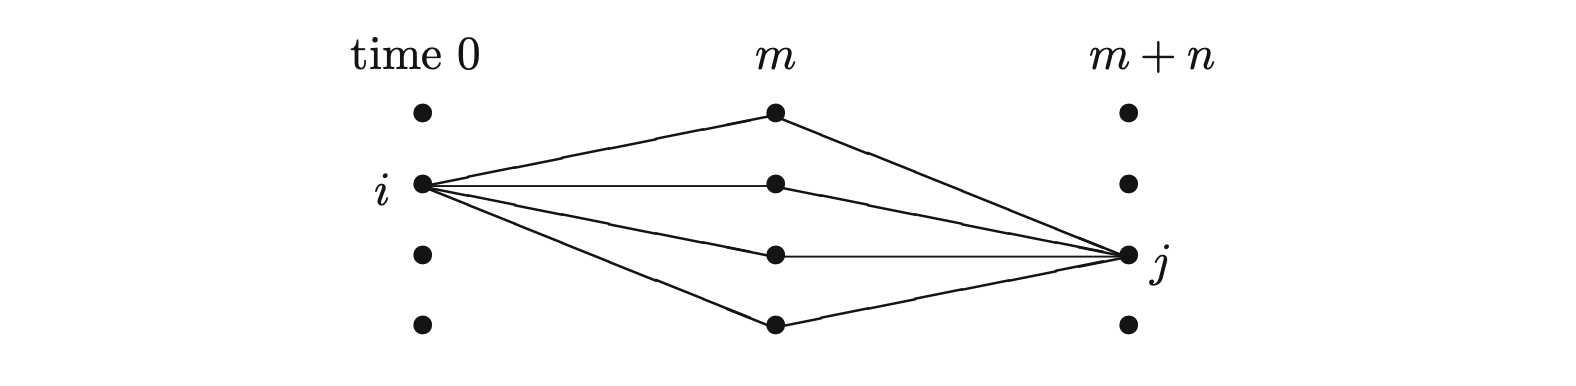
\includegraphics[width=0.9\textwidth]{figures/split_steps.png}
\end{figure}

\subsection{多步转移概率与矩阵乘法}

\begin{definition}
    设 $X=\{X_n,n\geq 0\}$ 为马氏链,称
    \[
    p_{ij}(m,m+n):=\PP(X_{n+m}=j|X_m=i)\quad (i,j\in S, m,n\geq 0)
    \]
    为 $X$ 的 $n$ 步转移概率,并称 $P(m,m+n)=(p_{ij}(m,m+n))_{i,j\in S}$ 为 $X$ 的 $n$ 步转移(概率)矩阵,其中
    \[
    p_{i,j}(0,0)=\delta_{ij}=\begin{cases}
        1 & i=j\\
        0 & i\neq j
    \end{cases}
    \]
\end{definition}

当 $X$ 时齐,$P(m,m+1)=(p_{ij}(m,m+1))_{i,j\in S}=(p_{ij}(0,1))_{i,j\in S}=(p_{ij})_{i,j\in S}$

可见 $n=1$ 时,$P(m,m+1)$ 与 $m$ 无关。那 $n>1$ 时呢?

\subsubsection{Chapman-Kolmogorov方程}

\begin{theorem}[C-K方程]\label{thm:CK}
    设 $\{X_n,x\geq 0\}$ 为马氏链
    \[
    p_{ij}(m,m+n+r)=\sum_{k\in S}p_{ik}(m,m+n)p_{kj}(m+n,m+n+r)
    \]
    其中 $i,j\in S,m,n,r\geq 0$,即
    \[
    P(m,m+n+r)=P(m,m+n)P(m+n,m+n+r)
    \]
\end{theorem}

\begin{figure}[H]
    \centering
    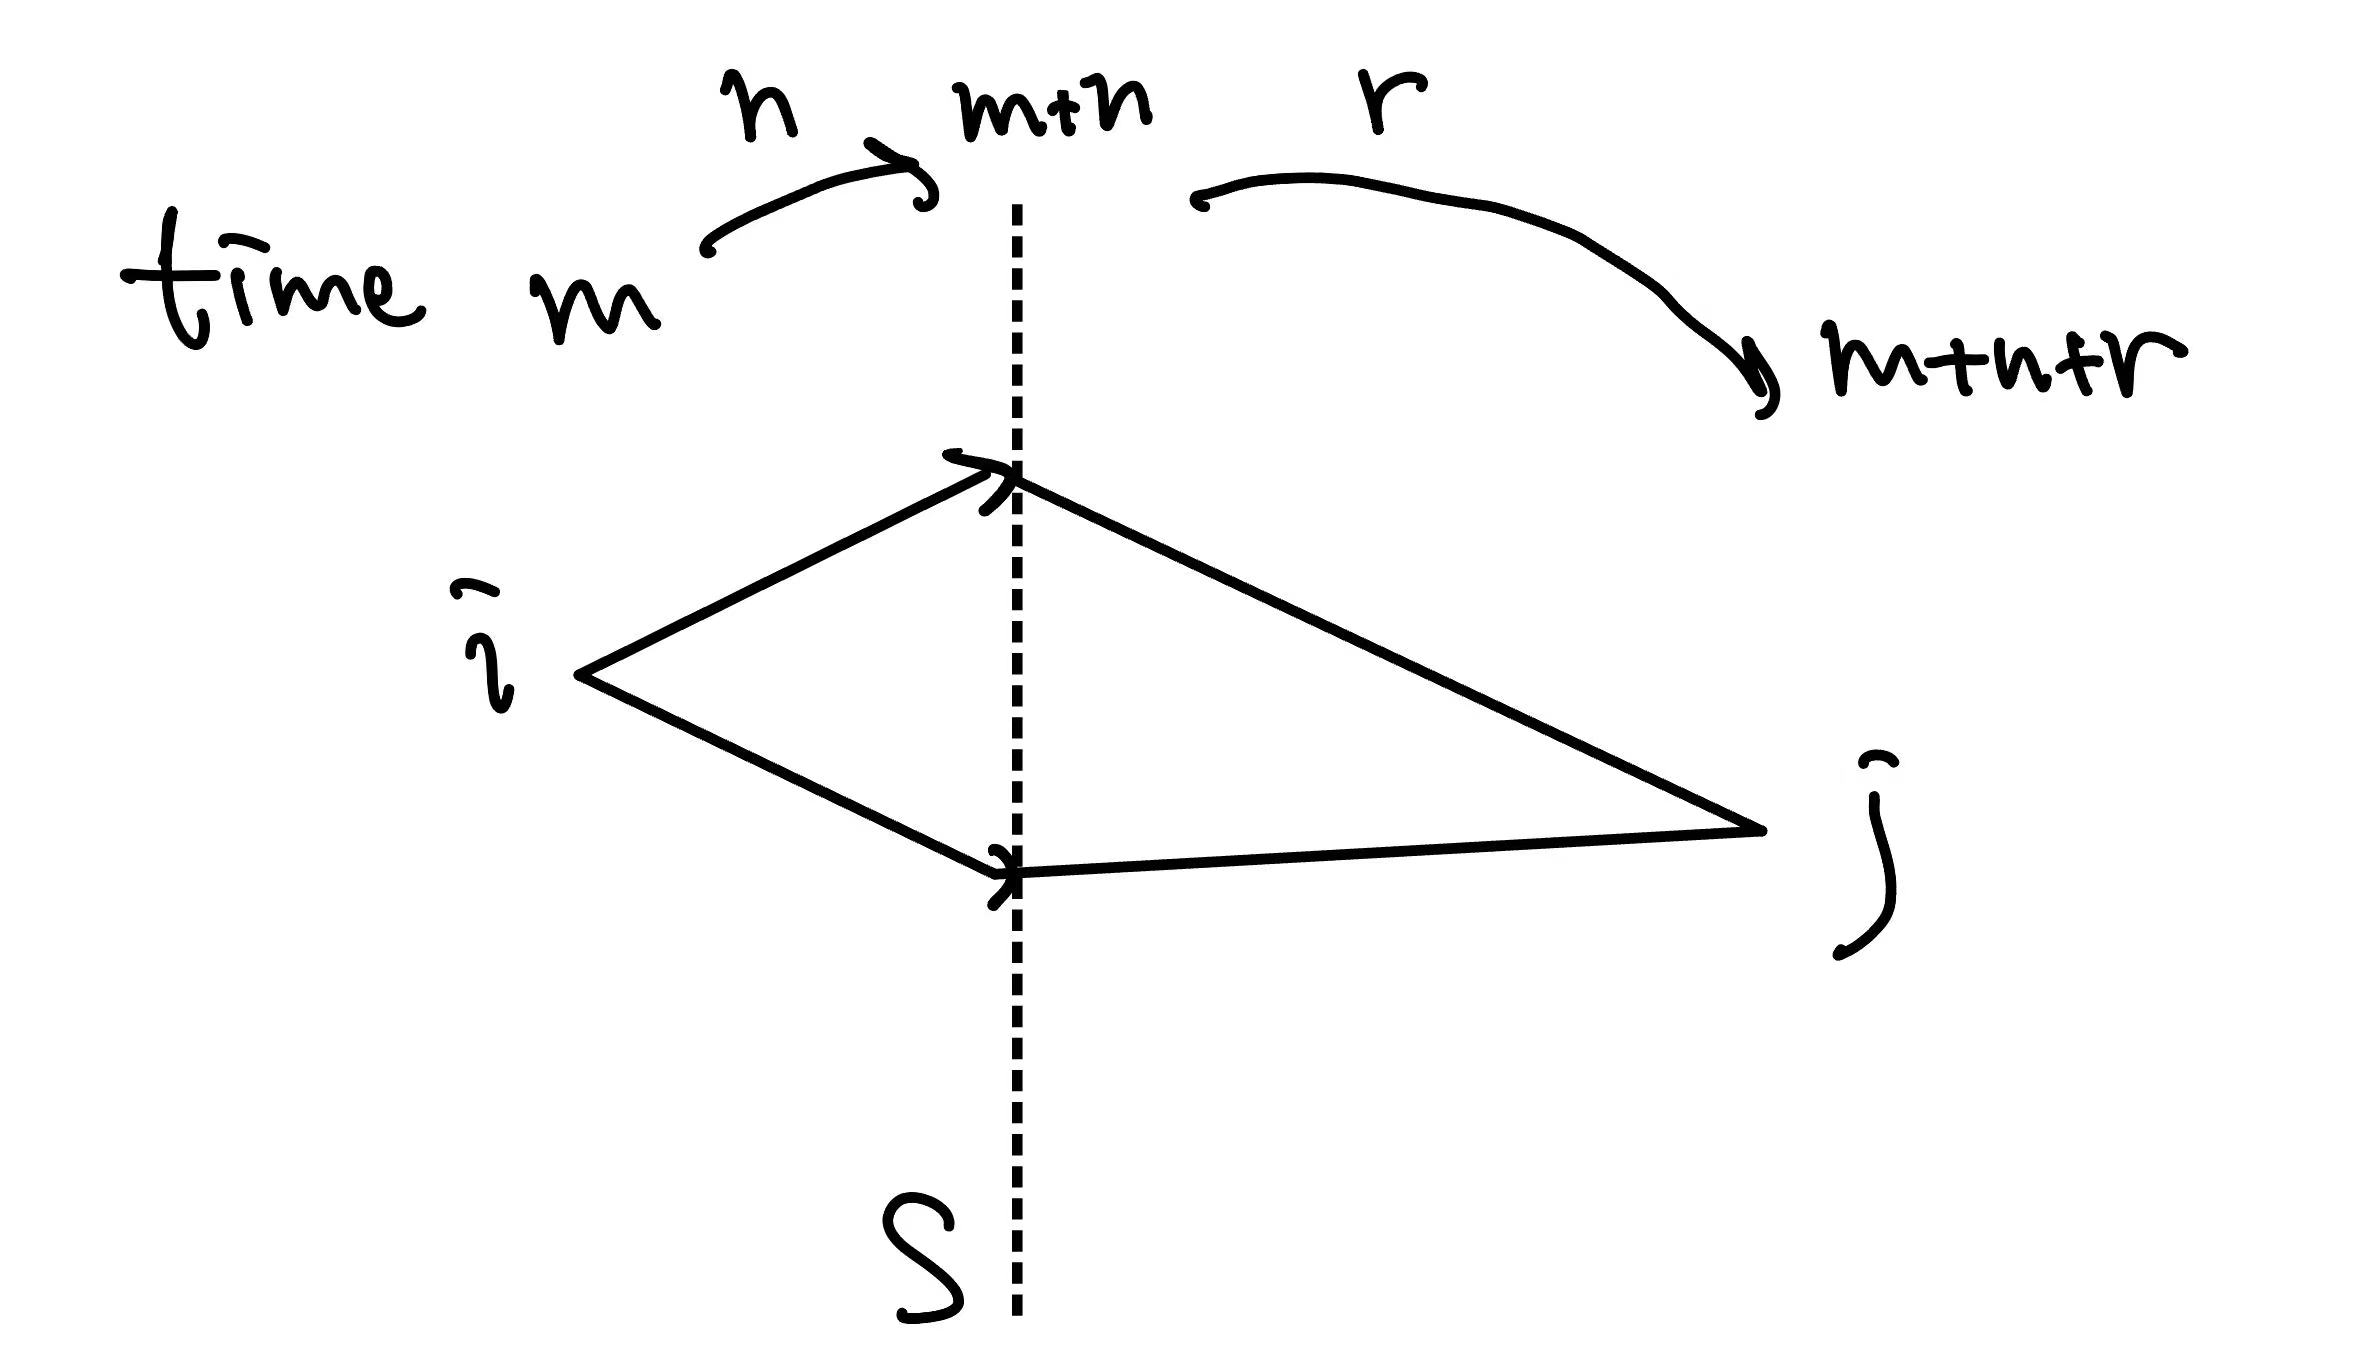
\includegraphics[width=0.55\textwidth]{figures/multi_steps.jpg}
    \caption{Multi-steps}
\end{figure}

证明:

\[
\begin{aligned}
    p_{ij}(m,m+n+r)&=P(X_{m+n+r}=j|X_m=i)\\
    &=\sum_{k\in S}P(X_{m+n+r}=j,X_{m+n}=k|X_m=i)\\
    &=\sum_{k\in S}\PP_{\{X_m=i\}}(X_{m+n+r}=j|X_{m+n}=k)\PP_{\{X_m=i\}}(X_{m+n}=k)\quad [\text{乘法公式}\eqref{eq:multiply_func}]\\
    &=\sum_{k\in S}p_{ik}(m,m+n)p_{kj}(m+n,m+n+r)\quad [\text{Markov}]
\end{aligned}
\]

\begin{corollary}
    设 $X$ 为具有(一步)转移矩阵 $P$ 的时齐马氏链,则
    \begin{enumerate}
        \item $\forall m,n\geq 0$,有 $P(m,m+n)=P(0,n)=P^n$。其中,约定 $P^0=I$(单位矩阵)
        
        从而,可记 $X$ 的 $n$ 步转移概率为 $p_{ij}(n)$ 或 $p_{ij}^{(n)}$,$n$ 步转移概率矩阵为 $P(n)$,且有
        \[
        P(n)=P^n=(p_{ij}^{(n)})_{i,j\in S}
        \]
        \item C-K 方程可改写为
        \[
        p_{ij}(m+n)=\sum_{k\in S}p_{ik}^{(m)}p_{kj}^{(n)}
        \]
        $P(m+n)=P(m)P(n)$,即 $P^{m+n}=P^m P^n$
    \end{enumerate}
\end{corollary}

证明:

\[
\begin{aligned}
    P(m,m+n)&=P(m,m+1)\cdot P(m+1,m+n)\quad [\text{C-K}]\\
    &=P\cdot P(m+1,m+n)\quad [\text{时齐}]\\
    &=P^n\qed
\end{aligned}
\]

\begin{proposition}
    $\forall n\geq 0, P(n)=P^n$ 仍是一个随机矩阵(定理\ref{thm:random_matrix})
\end{proposition}

证明:$n=2$时,$P^2=(p_{ij}(2))_{i,j\in S}$

$\Rightarrow$
\[
\begin{aligned}
    \sum_{j\in S}p_{ij}(2)&=\sum_{j\in S}\sum_{k\in S}p_{ik}p_{kj}\quad [\text{C-K}, \text{ 默认}p_{ik}(1)=p_{ik}]\\
    &=\sum_{k\in S}\sum_{j\in S}p_{ik}p_{kj}\\
    &=\sum_{k\in S}p_{ik}\cdot(\sum_{j\in S}p_{kj})\\
    &=\sum_{k\in S}p_{ik}=1\qed
\end{aligned}
\]
第二个等号,级数可交换是因为非负,要么有限(收敛)、要么$+\infty$(发散)

\subsubsection{马氏链的任意有限维分布}

\begin{proposition}
    $X\sim\text{Markov}(\mu, P)$,其中 $\mu=(\mu_i)_{i\in S}, P=(p_{ij})_{i,j\in S}$,则
    \[
    \PP(X_{u_1}=i_1,\cdots,X_{u_n}=i_n)=\mu_{i_1}^{(u_1)}\prod_{k=1}^{n-1}p_{i_k,i_{k+1}}^{(u_{k+1}-u_k)}
    \]
    其中,$0<u_1<u_2<\cdots<u_n$,$i_1,i_2,\cdots,i_n\in S$,$\mu^{(u_1)}=(\mu_i^{(u_1)})_{i\in S}$ 为 $X_{u_1}$ 的有限维分布
\end{proposition}

证明:
\[
\begin{aligned}
    \PP(X_{u_1}=i_1,\cdots,X_{u_n}=i_n)&=\PP(X_{u_1}=i_1)\cdot \PP(X_{u_2}=i_2|X_{u_1}=i_1)\cdots \PP(X_{u_n}=i_n|X_{u_1}=i_1,\cdots,X_{u_{n-1}}=i_{n-1})\\
    &=(\mu_{i_1}^{(u_1)})p_{i_1,i_2}^{(u_2-u_1)}\cdots p_{i_{n-1},i_n}^{(u_n-u_{n-1})}\quad [\text{Markov}]\\
    &=\mu_{i_1}^{(u_1)}\prod_{k=1}^{n-1}p_{i_k,i_{k+1}}^{(u_{k+1}-u_k)}
\end{aligned}
\]

用概率表示不够直观,尝试用转移矩阵来表示

\begin{lemma}
   $\mu^{(m+n)}=\mu^{(n)}P^m(\forall m,n\geq 0)$,即
   \[
   \mu_j^{(m+n)}=(\mu^{(n)}P^m)_j=\sum_{i\in S}\mu_i^{(n)}p_{ij}^{(m)}
   \]
   特别地,取 $n=0$,则 $\mu^{(m)}=\mu\cdot P^m$($\mu$看成行向量),即 $\mu_j^{(m)}=(\mu P^m)_j=\sum_{i\in S}\mu_i\cdot p_{ij}^{(m)}$
\end{lemma}

证明:
\[
\begin{aligned}
    \mu_j^{(n+m)}=\PP(X_{n+m}=j)&=\sum_{i\in S}\PP(X_{n+m}=j|X_n=i)\PP(X_n=i)\\
    &=\sum_{i\in S}p_{ij}(m)\mu_i^{(n)}\\
    &=(\mu^{(n)}P^m)_j\qed
\end{aligned}
\]

$\Rightarrow \mu^{(m+n)}=\mu^{(n)}P^m$

\begin{theorem}[任意有限维分布II]
    $\forall 0\leq u_1<u_2<\cdots<u_n, i_1,\cdots,i_n\in S$
    \[
    \PP(X_{u_1}=i_1,\cdots,X_{u_n}=i_n)=(\mu P^{u_1})_{i_1}\prod_{k=1}^{n-1}P_{i_k,i_{k+1}}^{u_{k+1}-u_k}
    \]
    其中,$P_{i,j}^m=:(P^m)_{i,j}=:p_{i,j}^{(m)}$
\end{theorem}

讨论随机过程地存在性:

抽象地,$\mu,P\xrightarrow{\text{定理}\eqref{thm:Kolmogorov}}\text{有限维分布族}\rightarrow X\sim \text{Markov}(\mu,P)$,$\mu,P$可以刻画具备对称性、相容性的有限维分布

具体地,参考Resnick\cite{resnick}, P62, Section 2.1 (\href{https://dafuzhuu.github.io/stochastic-process/pdf/Resnick.pdf}{PDF链接})

\subsection{(从固定点出发的)马氏链}

固定 $i\in S$,定义 $\PP_i(\cdot)=\PP(\cdot|X_0=i)$, $\EE_i(X)=\EE(X|X_0=i)=\sum_{x\in S}x\PP_i(X=x)$

\subsubsection{链的状态:常返和暂留}

\begin{definition}
    称状态 $i$ 为常返的,若
    \[
    \PP_i(X_n=i\text{对某个}n\geq 1)=1
    \]
    如果上面的概率$<1$,则称为暂留的/非常返的
\end{definition}

注:$i$ 常返 $\Leftrightarrow$ $\PP_i(\cup_{n\geq 1}\{X_n=i\})=1$

思考:$i$ 常返 $\Leftrightarrow$ “不停地/无数次回到$i$”

$\qquad \Leftrightarrow$ $\PP_i(\omega|\omega\in \text{无数多个} \{X_n=i\})$

$\qquad \Leftrightarrow$ $\PP_i(\omega|\omega\in\cap_{k\geq 1}\cup_{n\geq k}\{X_n=i\},\forall k)$

$\qquad \Leftrightarrow$ $\PP_i(X_n=i, i.o.)$ (infinitely often)

无数多次返回 $i$ 可严格定义为:
\[
\bigcap_{k\geq 1}\bigcup_{n\geq k}\{X_n=i\}
\]
集合的语言中,$\cup$即$\exists$,$\cap$即$\forall$,因此
\begin{itemize}
    \item $\bigcup_{n\geq k}\{X_n=i\}$ 表示 $\exists n_0\geq k$ 使得 $X_{n_0}=i$
    \item 对 $\forall k$ 取交集 $\bigcap_{k\geq 1}$,即无论 $k$ 多大,总存在更大的 $n$ 满足 $X_n=i$,从而保证无限次返回
\end{itemize}
即 $\forall k, \exists n_k, s.t. \{X_{n_k}=i\}$发生
\[
\begin{aligned}
    k=1&, n_1\geq k\\
    k=n_1+1&, n_2\geq n_1+1>n_1\\
    &\cdots
\end{aligned}
\]

\begin{remark}[如何进一步理解]
    无界和$\infty$的区别是什么?

无界:$\forall M>0,\exists k, s.t. |x_k|>M$
\begin{example}
    $1,2,3,4,\cdots$ 为 $\infty$/无界

    $1,0,2,0,3,0,4,\cdots$ 并非 $\infty$,但是无界的
\end{example}
迁移到$\bigcap_{k\geq 1}\bigcup_{n\geq k}$的例子
\begin{example}
    $A_1=\{0,1\},A_2=\{2\},A_3=\{0,3\},\cdots$,则
    \[
    \bigcap_{k=1}^{\infty}\bigcup_{n\geq k}A_n=\{0\},\qquad \bigcap_{k=1}^{\infty}A_k=\emp
    \]
    其中 $\bigcap_{k=1}^{\infty}\bigcup_{n\geq k}$ 也即 $\limsup$
\end{example}
\end{remark}

但我们推理得到的“常返”和定义里的并不等价
\[
\bigcap_{k\geq 1}\bigcup_{n\geq k}\{X_n=i\}\nLeftrightarrow \bigcup_{n\geq 1}\{X_n=i\}
\]
且LHS是RHS的子集,因此由定义的$\PP(RHS)=1$不能推出$\PP(LHS)=1$。于是我们疑惑为什么会叫它常返。这里要用到高阶知识“停时”,我们最后会回到这个问题。

下面给出几种判断常返/暂留的方法。

\subsubsection{从数学角度:并改写成不交并}

$i$ 常返 $\Leftrightarrow$ $\PP_i(\cup_{n\geq 1}\{X_n=i\})=1$

$\qquad \Leftrightarrow \PP_i(\text{有限步到达}i)=1$

$\qquad \Leftrightarrow \PP(\text{从}i\text{出发条件下,有限时间内回到}i)=1$

$B_1(i)=\{X_1=i\},B_2(i)=\{X_2=i\}\backslash \{X_1=i\}=\{X_2=i,X_1\neq i\},$ $\cdots,$ $B_n(i)=\{X_n=i,X_{n-1}\neq i\cdots,X_1\neq i\}$
\[
\Rightarrow\quad \sum_{n\geq 1}B_n(i)=\bigcup_{n\geq 1}\{X_n=i\} [\text{练习}\eqref{exer:disjoint_union}]
\]
$i$ 常返 $\Leftrightarrow$ $1=\PP_i(\sum_{n\geq 1}B_n(i))=\sum_{n\geq 1}\PP_i(B_n(i))$,第二个等号由可列可加性得到(定义\ref{def:prob_measure})
\[
\begin{aligned}
    \PP_i(B_n(j))&=\PP_i(X_n=j,X_{n-1}\neq j,\cdots,X_1\neq j)\\
    &=\PP_i(\text{首次访问}j\text{的时刻为}n)\\
    &=\PP_i(\text{走}n\text{步首次到达}j)
\end{aligned}
\]
故
\[
\begin{aligned}
    \PP_i(\sum_{n\geq 1}B_n(i))&=\PP_i(\text{首次访问}j\text{的时刻为有限时间})\\
    &=\PP_i(\text{有限时间内首次访问}j)
\end{aligned}
\]
记号
\[
f_{ij}:=\PP_i(\text{首次访问}j\text{的时刻为有限时间})
\]
\[
f_{ij}(n):=\PP_i(B_n(j))=\PP_i(\text{首次访问}j\text{的时刻为}n)
\]

\begin{proposition}
    常返和暂留的等价命题
    \begin{enumerate}
        \item $i$ 常返 $\Leftrightarrow$ $1=f_{ii}=\sum_{n\geq 1}f_{ii}(n)$
        \item $i$ 暂留 $\Leftrightarrow$ $1>f_{ii}=\sum_{n\geq 1}f_{ii}(n)$
    \end{enumerate}
\end{proposition}

\subsubsection{从“多步转移概率”角度判别}

定义新记号($P$不是转移矩阵)
\[
P_{ij}(s):=\sum_{n\geq 0}s^n p_{ij}(n)\qquad F_{ij}(s):=\sum_{n\geq 0}s^n f_{ij}(n)
\]
其中,$p_{ij}(0)=\delta_{ij},f_{ij}(0)=0$
\[
\delta_{ij}=\begin{cases}
    1 & i=j\\
    0 & i\neq j
\end{cases}
\]

注:当 $|s|<1$ 时,$P_{ij}(s),F_{ij}(s)$ 绝对收敛

由 Abel 连续性定理,
\[
\lim_{s\uparrow 1}F_{ij}(s)=\sum_{n\geq 1}f_{ij}(n)=f_{ij}\in [0,1]
\]
\[
\lim_{s\uparrow 1}P_{ij}(s)=\sum_{n\geq 0}p_{ij}(0)=\text{finite}/+\infty
\]
\begin{lemma}
    [Grimmett\cite{grimmett}, Thm 6.3.3] 设 $|s|<1$,则
    \[
    P_{ij}(s)=\delta_{ij}+P_{jj}(s)F_{ij}(s)
    \]
    其中
    \[
    \delta_{ij}=\begin{cases}
        1 & i=j\\
        0 & i\neq j
    \end{cases}
    \]
\end{lemma}

证明:构造不交并,$B_m(i)=\{X_m=i,X_{m-1}\neq i,\cdots,X_1\neq i\}, m\geq 1$

$\Rightarrow$ $\sum_{m\geq 1}B_m(i)=\cup_{n\geq 1}\{X_n=i\}, B_m(i)\st \{X_n\neq i\}, m\geq n+1$
\[
\begin{aligned}
    p_{ij}(n)=\PP_i(X_n=j)&=\PP_i(\{X_n=j\}\cap \sum_{m\geq 1}B_m(j))\\
    &=\sum_{m\geq 1}\PP_i(\{X_n=j\}\cap B_m(j))
    &=\sum_{m=1}^n\PP_i(\{X_n=j\}\cap B_m(j))
\end{aligned}
\]
最后一个等号成立是因为 $m\geq n+1$ 时 $\{X_n=j\}\cap B_m(j)$ 为空集
\[
\sum_{m=1}^n\PP_i(\{X_n=j\}\cap B_m(j))=\sum_{m=1}^n\PP_i(X_n=j|B_m(j))\PP_i(B_m(j))
\]
其中 $X_m=j,X_{n-1}\neq j,\cdots,X_1\neq j$,$X_{n-1}\in S\backslash \{j\}$

用一般而非单点的马氏性(引理\ref{lem:markov_equiv}$M_3$)
\[
\begin{aligned}
    \sum_{m=1}^n\PP_i(X_n=j|B_m(j))\PP_i(B_m(j))&=\sum_{m=1}^n\PP(X_n=j|X_m=j)\cdot f_{ij}(m)\\
    &=\sum_{m=1}^n p_{jj}(n-m)\cdot f_{ij}(m)
\end{aligned}
\]
当 $n\geq 1$ 时,
\[
\begin{aligned}
    P_{ij}(s)&=s^0p_{ij}(0)+\sum_{n\geq 1}s^n\cdot p_{ij}(n)\\
    &=\delta_{ij}+\sum_{n\geq 1}s^n\sum_{m=1}^n p_{jj}(n-m)f_{ij}(m)\\
    &=\delta_{ij}+\sum_{n\geq 1}\sum_{m=1}^n s^n p_{jj}(n-m)f_{ij}(m)\\
    &=\delta_{ij}+\sum_{n\geq 1}\sum_{m=1}^n(s^{n-m}p_{jj}(n-m))(s^m f_{ij}(m))\\
    &=\delta_{ij}+\sum_{n=1}^{\infty}\sum_{m=1}^{\infty}\II_{\{1\leq m\leq n\}}(s^{n-m}p_{jj}(n-m))(s^m f_{ij}(m))
\end{aligned}
\]
把 $\II_{\{1\leq m\leq n\}}(s^{n-m}p_{jj}(n-m))(s^m f_{ij}(m))$ 看作 $a_{n,m}$,由推论\ref{lem:abs_convergence}考察绝对收敛

$0\leq s<1, |s|=s$

正向级数一定有意义,就看是有限/$\infty$
\[
\begin{aligned}
    &\sum_{n=1}^{\infty}\sum_{m=1}^{\infty}\II_{\{1\leq m\leq n\}}s^{n-m}p_{jj}(n-m)s^m f_{ij}(m)\\
    =&\sum_{m=1}^{\infty}\sum_{n=1}^{\infty}\II_{\{1\leq m\leq n\}}s^{n-m}p_{jj}(n-m)s^m f_{ij}(m)\\
    =&\sum_{m=1}^{\infty}(\sum_{n=m}^{\infty}s^{n-m}p_{jj}(n-m))s^m f_{ij}(m)\\
    =&(\sum_{n=0}^{\infty}s^{n}p_{jj}(n))(\sum_{m=1}^{\infty}s^m f_{ij}(m))<\infty\quad [\text{变量代换}n\leftarrow n-m]
\end{aligned}
\]
因为 $s^0f_{ij}(0)=0$,则 $\sum_{m=0}^{\infty}s^m f_{ij}(m)=\sum_{m=1}^{\infty}s^m f_{ij}(m)$。代回原式
\[
P_{ij}(s)=\delta_{ij}+P_{jj}(s)\cdot F_{ij}(s)
\]

\begin{proposition}\label{prop:states_equiv}
    (1) $j$ 常返 $\Leftrightarrow$
    \[
        1=f_{jj}\Leftrightarrow \sum_{n\geq 0}p_{jj}(n)=\infty
    \]
    (2) $j$ 暂留 $\Leftrightarrow$
    \[
    \begin{aligned}
        1>f_{jj}&\Leftrightarrow \sum_{n\geq 0}p_{jj}(n)<\infty\\
        &\Rightarrow \sum_{n\geq 0}p_{ij}(n)<\infty, \forall i\in S\\
        &\Rightarrow \limit{n}p_{ij}(n)=0,\forall i\in S
    \end{aligned}
    \]
\end{proposition}

证明:只证(1). $|s|<1$时,$P_{ij}(s)=\delta_{ij}+P_{jj}(s)F_{ij}(s)$

$\Rightarrow P_{jj}(s)=1+P_{jj}(s)F_{jj}(s)$

$\Rightarrow$
\[
P_{jj}(s)=\frac{1}{1-F_{jj}(s)}\tag{*}
\]
$j$ 常返 $\Leftrightarrow$ $1=f_{jj}=F_{jj}(1)\overset{\text{Abel}}{=}\lim_{s\uparrow 1}F_{jj}(s)$

对 (*),令 $s\to 1$,有 $\sum_{n\geq 0}p_{jj}(n)=+\infty$

\begin{problem}[作业5-1]
证明:$j$ 暂留 $\Rightarrow \sum_{n\geq 0}p_{ij}(n)<\infty, \forall i\in S$
\end{problem}

\subsubsection{从“首次回访时间”角度判别}
\[
\begin{aligned}
    j\text{常返}&\Leftrightarrow 1=\PP_j(X_n=j\text{ 对某个}n\geq 1)=\PP_j(\text{有限时间内回访}j)\\
    &\Leftrightarrow 1=f_{jj}=\PP_j(\underbrace{\text{首次回访}j\text{的时刻}}_{T_j<\infty}\text{有限})\\
    &\quad =\sum_{n\geq 1}f_{jj}(n)=\sum_{n\geq 1}\PP_j(\underbrace{\text{首次回访}j\text{的时刻}}_{T_j=n}\text{是}n)
\end{aligned}
\]
\begin{definition}
    首次回访$j$的时刻
    \[
    T_j=\min\{n\geq 1|X_n=j\}
    \]
    约定 $\min \emp=+\infty$
\end{definition}

注:$\{T_j=\infty\}\Leftrightarrow \{\omega|\{n\geq 1|X_n(\omega)=j\}=\emp\}$

$\quad \Leftrightarrow \{\omega|X_n(\omega)\neq j,\forall n\geq 1\}=\cap_{n\geq 1}\{X_n\neq j\}$

\begin{property}
    $f_{jj}=\PP_j(T_j<\infty), f_{jj}(n)=\PP_j(T_j=n)$
\end{property}

定义 $\PP_j(T_j<\infty)=\rho_{jj}$

\begin{proposition}
    联系命题\ref{prop:states_equiv}
    \begin{enumerate}
        \item $j$ 常返 $\Leftrightarrow$ $1=\rho_{jj}=\PP_j(T_j<\infty)\Leftrightarrow 0=\PP_j(T_j=\infty)$
        \item $j$ 暂留 $\Leftrightarrow$ $1>\rho_{jj}=\PP_j(T_j<\infty)\Leftrightarrow 0<\PP_j(T_j=\infty)$
    \end{enumerate}
\end{proposition}

\begin{definition}
    $j$ 的平均回访时间
    \[
    m_j:=\EE_jT_j=\EE(T_j|X_0=j)
    \]
\end{definition}

\begin{theorem}
    \[
    m_j=\EE_j T_j=\begin{cases}
        \sum_{n\geq 1}nf_{jj}(n) & j\text{常返}\\
        \infty & j\text{暂留}
    \end{cases}
    \]
\end{theorem}

证明:

(1) $j$暂留 $\Rightarrow$ $\PP_j(T_j=\infty)>0$

$\quad \Rightarrow \EE T_j=\EE T_j\II_{\{T_j=\infty\}}+\EE T_j\II_{\{T_j<\infty\}}\geq \EE T_j\II_{\{T_j=\infty\}}=\infty\cdot \PP_{T_j=\infty}=\infty$

(2) $j$常返 $\Rightarrow$ $\PP_j(T_j=\infty)=0$

取期望时不起作用,因为 $0\cdot \infty$ 是不定形
\[
\begin{aligned}
    \EE_j T_j&=\EE_j T_j\II_{\{T_j<\infty\}}\\
    &=\EE_j T_j\II_{\sum_{n\geq 1}\{T_j=n\}}\\
    &=\EE_j\sum_{n\geq 1}T_j\II_{\{T_j=n\}}\quad [\text{定义\eqref{def:discrete_rv}}]\\
    &=\sum_{n\geq 1}n\PP_j(T_j=n)\\
    &=\sum_{n\geq 1}n f_{jj}(n)
\end{aligned}
\]
\begin{definition}
    $j$常返时
    \begin{enumerate}
        \item $\EE_j T_j<\infty$ 称$j$是正常返
        \item $\EE_j T_j=\infty$ 称$j$是零常返(平均意义上再也不回来)
    \end{enumerate}
\end{definition}

$j$ 常返 $\Leftrightarrow 1=f_{jj}\Leftrightarrow \sum_{n\geq 0}p_{jj}(n)=\infty$

$\Leftrightarrow 1=\rho_{jj}=\PP_j(T_j<\infty)\Leftrightarrow 0=\PP_j(T_j=\infty)$
\[
\begin{aligned}
    \PP_j(T_j<\infty)&=\PP(\text{从}j\text{出发条件下,首次回到}j\text{的时刻有限})\\
    &=\PP(\text{从}j\text{出发条件下,有限时间内至少访问}j\text{有1次})\\
    &=\PP(\text{从}j\text{出发条件下,有限时间内回访}j\text{的次数}\geq 1)
\end{aligned}
\]

\begin{definition}
    链在时刻$0$之后,访问$j$的次数
    \[
    N(j):=\# \{n\geq 1|X_n=j\}=\sum_{n\geq 1}\II_{X_n=j}
    \]
\end{definition}

注:$N(j):\Omega\to \{0,1,2,\cdots\}\cup \{+\infty\}$

至此,做个阶段性小结,回顾 $i$ 常返的几种等价表示
\[
\begin{aligned}
    i\text{常返} &\overset{\text{Def}}{\Leftrightarrow}1=\PP_i(\bigcup_{n\geq 1}\{X_n=i\})\\
    &\Leftrightarrow 1=f_{ii}:=\sum_{n\geq 1}f_{ii}(n)=\sum_{n\geq 1}\PP_i(X_1\neq i,\cdots, X_{n-1}\neq i,X_n=i)\Leftrightarrow \sum_{n\geq 1}p_{ii}(n)=\infty\\
    &\Leftrightarrow 1=\rho_{ii}=\PP_i(T_i^{(1)}:=T_i<\infty)=\PP_i\{N(i)\geq 1\}=1
\end{aligned}
\]

无数次地回访 $\leftrightarrow$ 访问次数$=\infty$ $\leftrightarrow$ $\PP_i(N(i):=\sum_{n\geq 1}\II_{\{X_n=i\}}=\infty)=1$

两种表述的等价条件互相等价吗?即
\[
\PP_i(N(i)\geq 1)\overset{?}{\Leftrightarrow} \PP_i(N(i)=\infty)=1
\]
需要 Strong Markov Property (SMP) 使上面$\Leftrightarrow$成立。这里先补充一些关于 $N(j)$ 的内容,然后再回到证明。

考察 $\{N(y)=\infty\}=\cap_{k\geq 1}\{N(y)\geq k\}$

由概率测度的连续性(性质\ref{prt:measure_continuity})
\[
    \PP_x(N(y)=\infty)=\limit{k}\PP_x(N(y)\geq k)
\]
其中,
\[
\begin{aligned}
    \PP_x(N(y)\geq k) &= \PP(\text{从}x\text{出发条件下,访问}y\text{的次数}\geq k)\\
    &=\PP(\text{从}x\text{出发条件下,至少访问}y\text{有}k\text{次})\\
    &=\PP(\text{从}x\text{出发条件下,第}k\text{次访问}y\text{的时刻有限})
\end{aligned}
\]
$T_y^{(1)}:=T_y:=\min\{n\geq 1|X_n=y\}$

$T_y^{(2)}:=\min\{n>T_y^{(1)}|X_n=y\}$

$\quad \vdots$

$T_y^{(k)}:=\min\{n>T_y^{(k-1)}|X_n=y\}, \forall k\geq 2$
\[
\Rightarrow \quad \PP_x(N(y)\geq k)=\PP_x(T_y^{(k)}<\infty)
\]

\begin{definition}
    第$k$次访问概率
    \[
    \rho_{xy}^{(k)}:=\PP_x(T_y^{(k)}<\infty)
    \]
    其中,$\rho_{xy}^{(1)}=\rho_{xy}$
    
    第$k$次回访概率
    \[
    \rho_{yy}^{(k)}:=\PP_y(T_y^{(k)}<\infty)
    \]
\end{definition}

注:$\rho_{yy}^{(2)}\overset{?}{=}\rho_{yy}\cdot \rho_{yy}$

直观上是这样,但严格证明要求SMP

这是因为不同时间对应的是不同的随机过程,如
\begin{itemize}
    \item $t=0$时,过程是$\{X_n,n\geq 0\}$
    \item $t=T_j$时,过程是$\{X_{T_j+n},n\geq 0\}$
\end{itemize}
SMP是一个使得 $X_{T_j+n}=X_n,\forall T_j$ 的性质,之后会详细说。以上结论可总结成下面引理。

\begin{lemma}
    (由SMP知) $\rho_{xy}^{(k)}=\rho_{xy}\rho_{yy}^{(k-1)}$

    特别地,$\rho_{yy}^{(k)}=\rho_{yy}^k$
\end{lemma}

接着我们回到证明
\[
    \PP_i(N(i)\geq 1)=1 \Leftrightarrow \PP_i(N(i)=\infty)=1
\]

证明:$\Leftarrow$ 显然,因为 $\{N(i)=\infty\}$ 相对 $N(i)\geq 1$ 是小集合

$\Rightarrow$
\[
\PP_i(N(i)=\infty)=\limit{k}\PP_i(N(i)\geq k)\overset{\text{SMP}}{=}\limit{k}\rho_{ii}^k=1
\]
暂留的证明同理:
\[
\begin{aligned}
    i\text{暂留}&\Leftrightarrow \PP_i(N(i)=\infty)=\limit{k}\rho_{ii}^k=0\\
    &\Leftrightarrow 1> \rho_{ii}
\end{aligned}
\]

\subsubsection{从“平均回访次数”角度判别}

\[
N(y)=\sum_{n\geq 1}\II_{\{X_n=y\}}=\sum_{k\geq 1}\II_{\{N(y)\geq k\}}
\]
\begin{lemma}[Durrett\cite{durrett}, lem 1.11]
    \[
    \EE_yN(y)=\begin{cases}
        \infty & y\text{常返}\\
        \frac{\rho_{yy}}{1-\rho_{yy}} & y\text{暂留}
    \end{cases}
    \]
\end{lemma}

证明:
\[
\begin{aligned}
    \EE_yN(y)&=\EE_y\sum_{k\geq 1}\II_{\{N(y)\geq k\}}\overset{\text{Exa\eqref{exa:expec_of_indica}}}{=}\sum_{k\geq 1}\PP(N(y)\geq k)=\sum_{k\geq 1}\PP_y(T_y^{(k)}<\infty)\\
    &=\sum_{k\geq 1}\rho_{yy}^{(k)}\overset{\text{SMP}}{=}\sum_{k\geq 1}\rho_{yy}^k
\end{aligned}
\]
$\rho_{yy}=1\Rightarrow \EE_yN(y)=\infty$

$\rho_{yy}<1\Rightarrow \EE_yN(y)=\rho_{yy}/(1-\rho_{yy})$

下面证:$i$常返 $\Leftrightarrow$ $\EE_i N(i)=\infty$,也就是证 $\PP_i(N(i)=\infty)=1\Leftrightarrow \EE_i N(i)=\infty$

证明:$\Rightarrow$ 显然

$\Leftarrow$ $N(y)$ 为非负r.v.,有当$k\to\infty$时,$\forall \omega, \sum_{n=1}^k\II_{\{X_n=y\}}(\omega)\uparrow \sum_{n=1}^{\infty}\II_{\{X_n=y\}}(\omega)$
\[
\begin{aligned}
    \EE_yN(y)&:=\limit{k}\EE_y\sum_{n=1}^k\II_{X_n=y}\\
    &=\limit{k}\sum_{n=1}^k\EE_y\II_{\{X_n=y\}}\\
    &=\limit{k}\sum_{n=1}^k\PP_y(X_n=y)=\sum_{n=1}^{\infty}p_{yy}(n)
\end{aligned}
\]
将上面几个角度总结成下面定理
\begin{theorem}[链的状态:等价表述]\label{thm:states_equiv}
\[
\begin{aligned}
    i\text{常返} &\overset{\text{Def}}{\Leftrightarrow}1=\PP_i(\bigcup_{n\geq 1}\{X_n=i\})\quad [\text{回访发生的概率}]\\
    &\Leftrightarrow 1=f_{ii}:=\sum_{n\geq 1}f_{ii}(n)=\sum_{n\geq 1}\PP_i(X_1\neq i,\cdots, X_{n-1}\neq i,X_n=i)\Leftrightarrow \sum_{n\geq 1}p_{ii}(n)=\infty\quad [\text{首次回访发生}]\\
    &\Leftrightarrow 1=\rho_{ii}=\PP_i(T_i^{(1)}:=T_i<\infty)=\PP_i\{N(i)\geq 1\}=1\\
    &\overset{\text{why the name}}{\Leftrightarrow} \PP_i(N(i)=\infty)=\limit{k}\PP_i(N(i)\geq k)\overset{\text{SMP}}{=}\limit{k}\rho_{ii}^k=1\\
    &\Leftrightarrow \EE_i N(i)=\infty
\end{aligned}
\]
\end{theorem}

\subsubsection{停时与强马氏性}

\begin{definition}[停时/Stopping time]
    随机变量 $\tau:\Omega\to \{0,1,2,\cdots\}\cup\{+\infty\}$,满足 $\forall \infty>n\geq 0, \{\tau=n\}\in \sigma(X_0,\cdots,X_n)$,称 $\tau$ 是关于 $(X_n)_{n\geq 0}$ 的停时
\end{definition}

\begin{example}
首次回访时刻是一个停时

    $T_y^{(1)}:=T_y:=\min\{n\geq 1|X_n=y\}$
    \[
    \begin{aligned}
        \{T_y^{(1)}=n\} &=\{X_1\neq y,\cdots,X_{n-1}\neq y,X_n=y\}\quad n\geq 1\\
        &=\{(X_0,X_1,\cdots,X_n)\in S\times(S\backslash \{y\})\times\cdots\times(S\backslash \{y\})\times \{y\}\}\\
        &\in \sigma(X_0,\cdots,X_n)=(X_0,\cdots,X_n)^{-1}(\bigotimes_{n+1}2^S)
    \end{aligned}
    \]
\end{example}

\begin{definition}[停止$\sigma$代数]
    $\tau$是关于 $(X_n)_{n\geq 0}$ 的停时,定义
    \[
    \CF_{\tau}:=\{A|A\cap\{\tau=n\}\in\sigma(X_0,\cdots,X_n),\forall n\}
    \]
\end{definition}

注:$B\in \CF_i\Leftrightarrow B$是由$X_0,\cdots,X_{\tau}$决定的事件(这是直观上的解释,因为$\tau$是随机的,我们不知道“$\cdots$”是什么)

停时 $\sigma$-代数的定义是为了形式化“到随机时间 $\tau$ 为止的信息”。因为 $\tau$ 本身是随机的,我们不能直接写 $\sigma(X_0,\cdots,X_{\tau})$(因为 $\tau$ 不确定),所以需要通过对所有可能的 $\tau=n$ 进行分解。

$\quad \Leftrightarrow B\cap\{T=n\}\in \sigma(X_0,\cdots,X_n),\forall n$

\begin{problem}[作业5-2]
设 $\tau$ 为关于 $(X_n)_{n\geq 0}$ 的停时,即对任意的 $\infty>n\geq 0$,有
\[
\{\tau=n\}\in\sigma(X_0,\cdots,X_n)
\]
证明:
\begin{enumerate}
\item (停止$\sigma$代数的定义) $\CF_{\tau}:=\{A|A\cap \{\tau=n\}\in \sigma(X_0,\cdots,X_n),\forall n\geq 1\}$ 是一个$\sigma$-代数
\item $\sigma(X_{\tau})\in \CF_{\tau}$
\end{enumerate}
\end{problem}


\begin{lemma}[马氏性的小推广]\label{lem:markov_extend}
若 \( X \) 为马氏链,则对任意 \( n,m \geq 0, x_n \in S, A \in \otimes_{n+1}2^S, B \in \otimes_{m+1}2^S \)(即 \( A \subset S^{n+1}, B \subset S^{m+1} \)),有
\begin{equation}
\begin{aligned}
&P_{\{X_n=x_n\}}((X_0, \cdots , X_n) \in A, (X_n, \cdots , X_{n+m}) \in B)\\
=&P_{\{X_n=x_n\}}((X_0, \cdots , X_n) \in A) \times P_{\{X_n=x_n\}}((X_n, \cdots , X_{n+m}) \in B)
\end{aligned}
\label{eq:markov_extend}
\end{equation}
即 \((X_0, \cdots , X_n) \perp \!\!\! \perp_{\{X_n=x_n\}} (X_n, \cdots , X_{n+m})\) 的定义
\end{lemma}

证明:回顾马氏性\eqref{eq:markov_equiv_condition_M2}

不妨设 \( A = A_0 \times \cdots \times A_n, B = B_0 \times \cdots \times B_{n+m} \)

(Case 1) 若 \( x_n \notin A_n \) 或 \( x_n \notin B_0 \),则
\[
P_{\{X_n=x_n\}}((X_0, \cdots , X_n) \in A) = 0 \text{ 或 } P_{\{X_n=x_n\}}((X_n, \cdots , X_{n+m}) \in B) = 0
\]
且
\[
P_{\{X_n=x_n\}}((X_0, \cdots , X_n) \in A, (X_n, \cdots , X_{n+m}) \in B) = 0
\]
从而,\eqref{eq:markov_extend} 得证

(Case 2) 设 \( x_n \in A_n \),且 \( x_n \in B_0 \)。若 \( n = 0, m = 0 \),则显然有
\[
P_{\{X_n=x_n\}}((X_0, \cdots , X_n) \in A) = P_{\{X_n=x_n\}}((X_n, \cdots , X_{n+m}) \in B) = 1
\]
\[
P_{\{X_n=x_n\}}((X_0, \cdots , X_n) \in A, (X_n, \cdots , X_{n+m}) \in B) = 1
\]
此时,显然有 \eqref{eq:markov_extend} 成立。若 \( n \geq 1, m \geq 1 \),则
\[
P_{\{X_n=x_n\}}((X_0, \cdots , X_n) \in A) = P_{\{X_n=x_n\}} \left\{ X_j \in A_j, 0 \leq j \leq n-1 \right\}
\]
\[
P_{\{X_n=x_n\}}((X_n, \cdots , X_{n+m}) \in B) = P_{\{X_n=x_n\}} \left\{ X_j \in B_j, n+1 \leq j \leq n+m \right\}
\]
且
\[
\begin{aligned}
&P_{\{X_n=x_n\}}((X_0, \cdots , X_n) \in A, (X_n, \cdots , X_{n+m}) \in B)\\ =& P_{\{X_n=x_n\}} \left\{ X_j \in A_j, 0 \leq j \leq n-1, X_k \in B_k, n+1 \leq k \leq n+m \right\}\\
=& P_{\{X_n=x_n\}} \left\{ X_j \in A_j, 0 \leq j \leq n-1 \right\} P_{\{X_n=x_n\}} \left\{ X_k \in B_k, n+1 \leq k \leq n+m \right\}
\end{aligned}
\]
故而 \eqref{eq:markov_extend} 得证。对于其他情形 \( n \geq 1, m = 0 \) 或 \( n = 0, m \geq 1 \),可类似证明。\qed

\begin{proposition}[强马氏性]
    $X:=\{X_n,n\geq 0\}\sim \text{Markov}(\mu,P)$,$\tau$是关于$(X_n)_{n\geq 0}$的停时,则
    \begin{enumerate}
        \item 在$\{\tau<\infty\}$和$\{X_{\tau}=x\}$条件下
        \[
        (X_{\tau+n})_{n\geq 0}\sim\text{Markov}(\delta_x,P)
        \]
        其中 $\delta_x=(\delta_{xy})_{y\in S}$,记号
        \[
        \delta_{xy}=\begin{cases}
            1 & y=x\\
            0 & y\neq x
        \end{cases}
        \]
        注:$(X_{\tau+n})_{n\geq 0}\sim \text{Markov}(\delta_x,P)$ under $\PP(\cdot|\tau<\infty,X_{\tau}=x)$。在原先的概率测度 $\PP$ 下, $(X_{\tau+n})_{n\geq 0}$ 不是马氏链
        \item $\forall J\st \NN_0, \#J<\infty$,有
        \[
        \sigma(X_{\tau+n},n\in J)\ind_{\{\tau<\infty,X_{\tau}=x\}}\CF_{\tau}
        \]
        注:\begin{enumerate}
            \item $(X_{\tau+n})_{n\geq 0}$与$X_0,\cdots,X_{\tau}$独立
            \item $(X_{\tau+n})_{n\geq 0}\ind \CF_{\tau}$ under $\PP(\cdot|\tau<\infty,X_{\tau}=x)$
        \end{enumerate}
    \end{enumerate}
\end{proposition}

证明:(1) 回顾命题\ref{prop:markov_dist},

根据此结论,我们只需考察链 \(\{X_{\tau + n}, n \geq 0\}\) 的有限维分布。

(Step 1) 设 \(j_0 \neq x\)。则对任意的 \(n \geq 1, m \geq 0\),有
\[
\PP(X_{\tau + 0} = j_0, \cdots, X_{\tau + n} = j_n, \tau = m, X_\tau = x) = 0
\]
关于 \(m \geq 0\) 求和,并注意到 \(\{\tau < \infty\} = \sum_{m=0}^{\infty} \{\tau = m\}\),得:
\[
\PP(X_{\tau + 0} = j_0, \cdots, X_{\tau + n} = j_n, \tau < \infty, X_\tau = x) = 0
\]
两边同除 \(P(\tau < \infty, X_\tau = x)\),有
\[
\PP(X_{\tau + 0} = j_0, \cdots, X_{\tau + n} = j_n | \tau < \infty, X_\tau = x) = 0 = \delta_{x j_0} \prod_{k=0}^{n-1} p_{j_k j_{k+1}}
\]

(Step 2) 设 \(j_0 = x\)。注意到,对任意的 \(m \geq 0\),有
\[
\{\tau = m\} \in \sigma(X_0, \cdots, X_m)
\]
故而,由引理\ref{lem:markov_extend}知:对任意的 \(n \geq 1, m \geq 0\),有
\[
\{\tau = m\} \ind_{\{X_m = x\}} \{X_m = j_0, X_{m+1} = j_1, \cdots, X_{m+n} = j_n\}
\]
从而,对任意的 \(m \geq 0\),有
\[
\begin{aligned}
\PP(X_{\tau + 0} = j_0, \tau = m, X_\tau = x) &= P(X_{m + 0} = j_0, \tau = m, X_m = x)\\
&=\PP(X_{m + 0} = j_0, \tau = m| X_m = x) \times \PP(X_m = x)\quad [\text{乘法公式}\eqref{eq:multiply_func}]\\
&=\PP(X_{m + 0} = j_0 | X_m = x) \times \PP(\tau=m|X_m = x)\times \PP(X_m=x)\quad [\text{马氏性}\eqref{eq:M1}]\\
&=1\times \PP(\tau=m,X_m=x)\quad [\text{乘法公式}\eqref{eq:multiply_func}]\\
&=\delta_{xx}\PP(\tau=m,X_m=x)
\end{aligned}
\]
以及,对任意的 \(n \geq 1, m \geq 0\),有
\[
\begin{aligned}
&\PP(X_{\tau + 0} = j_0, X_{\tau + 1} = j_1, \cdots, X_{\tau + n} = j_n, \tau = m, X_\tau = x)\\
=& \PP(X_{m + 1} = j_1, \cdots, X_{m + n} = j_n, \tau = m, X_m = x)\\
=& \PP(X_{m + 1} = j_1, \cdots, X_{m + n} = j_n, \tau = m | X_m = x) \times \PP(X_m = x)\quad [\text{乘法公式}\eqref{eq:multiply_func}]\\
=& \PP(X_{m + 1} = j_1, \cdots, X_{m + n} = j_n | X_m = x) \times \PP(\tau=m|X_m = x)\times \PP(X_m=x)\quad [\text{马氏性}\eqref{eq:M1}]\\
=& \frac{\PP(X_{m + 1} = j_1, \cdots, X_{m + n} = j_n , X_m = x)}{\PP(X_m=x)}\times \PP(\tau=m|X_m = x)\times \PP(X_m=x)\\
=&\frac{\mu_x^{(m)}p_{x,j_1}p_{j_2,j_3}\cdots p_{j_{n-1},j_n}}{\mu_x^{(m)}}\times \PP(\tau=m,X_m=x)\quad [\text{马氏链}X\text{的有限维分布}\eqref{eq:markov_dist}]\\
=&\delta_{xx}p_{x,j_1}p_{j_2,j_3}\cdots p_{j_{n-1},j_n}\times \PP(\tau=m,X_m=x)
\end{aligned}
\]
其中,\(\mu_x^{(m)} := P(X_m = x)\)。综上,关于 \(m \geq 0\) 求和(注意到 \(\{\tau < \infty\} = \sum_{m=0}^{\infty} \{\tau = m\}\)),再两边同除以 \(P(\tau < \infty, X_\tau = x)\),得:当 \(j_0 = x\),对任意的 \(n \geq 0\),有
\[
\PP(X_{\tau + 0} = j_0, \cdots, X_{\tau + n} = j_n | \tau < \infty, X_\tau = x) = \delta_{x j_0} \prod_{k=0}^{n-1} p_{j_k j_{k+1}}.
\]

(Step 3) 综上,链的 \((X_{\tau + n})_{n \geq 0}\) 的有限维分布为
\[
\PP(X_{\tau + 0} = j_0, \cdots, X_{\tau + n} = j_n | \tau < \infty, X_\tau = x) = \delta_{x j_0} \prod_{k=0}^{n-1} p_{j_k j_{k+1}}.
\]
即有 \((X_{\tau + n})_{n \geq 0} \sim \text{Markov}(\delta_x, P)\) under $\PP(\cdot|\tau=\infty,X_{\tau}=x)$.

(2) 作业。

\begin{problem}[作业5-3]
$\forall J\st \NN_0, \#J<\infty$,有
\[
\sigma(X_{\tau+n},n\in J)\ind_{\{\tau<\infty,X_{\tau}=x\}}\CF_{\tau}
\]
注:\begin{enumerate}
    \item $(X_{\tau+n})_{n\geq 0}$与$X_0,\cdots,X_{\tau}$独立
    \item $(X_{\tau+n})_{n\geq 0}\ind \CF_{\tau}$ under $\PP(\cdot|\tau<\infty,X_{\tau}=x)$
\end{enumerate}
\end{problem}

用下面方法表述两次返回之间的等待时间 $S_y^{(k)}$

$T_y^{(0)}:=0, T_y^{(1)}:=T_y$,对于 $k\geq 2, T_y^{(k)}:=\min\{n\geq T_{y+1}^{(k-1)}|X_n=y\}$
\[
S_y^{(k)}=\begin{cases}
    T_y^{(k)}-T_y^{(k-1)}&\text{若 }T_y^{(k-1)}<\infty\\
    0 & \text{否则}
\end{cases}
\]
注意到 $T_y^{(k)}=T_y^{(k-1)}+\min\{n\geq 1|X_{T_y^{(k-1)}+n}=y\}$
\[
\Rightarrow S_y^{(k)}=\min\{n\geq 1|X_{T_y^{(k-1)}+n}=y\}, \text{if }T_y^{(k-1)}<\infty
\]
即 $(X_{T_y^{(k-1)}+n})_{n\geq 0}$ 的首次回访时刻 $S_y^{(k)}$

\begin{lemma}
    对 $k\geq 2$,有 $\sigma(S_y^{(k)})\ind_{\{T_y^{(k-1)}<\infty\}}\CF_{T_y^{(k-1)}}$,且\
    \[
    \PP(S_y^{(k)}<\infty|T_y^{(k-1)}<\infty)=\PP(T_y^{(1)}<\infty|X_0=y)=:\rho_{yy}
    \]
\end{lemma}

\begin{corollary}
    对 $k\geq 0$ 有 $\rho_{yy}^{(k)}=\rho_{yy}^k$,即
    \[
    \PP_y(N(y)\geq k)=\PP_y(T_y^{(k)}<\infty)=\rho_{yy}^k
    \]
\end{corollary}

\subsection{类结构}
\subsubsection{状态$i$间的关系:可达与互通}

\begin{definition}[可达]
    $i,j\in S$,若 $\exists n\geq 0, s.t.\quad p_{ij}(n)>0$,则称 $i$ 可达 $j$,记作 $i\to j$

    注:$i\to i,p_{ii}(0)=1>0$ 包括在内
\end{definition}

\begin{definition}[互通]
    若 $i\to j,j\to i$ 称 $i$ 与 $j$ 互通,记作 $i\leftrightarrow j$
\end{definition}

\begin{theorem}\label{thm:commu_equiv}
    对不同的 $i$ 与 $j$,下面命题等价
    \begin{enumerate}
        \item $i\to j$
        \item $0<f_{ij}=\rho_{ij}=\PP_i(T_j<\infty)$ [Durrett\cite{durrett}]
        \item $\exists$某些状态,$i_0=i,i_1,\cdots,i_{n-1},i_n=j,s.t.\quad p_{i_0,i_1}\cdots p_{i_{n-1},i_n}>0$
        \item $\PP_i(\exists n\geq 0,X_n=j)>0$
    \end{enumerate}
\end{theorem}

\begin{problem}[作业6-1]
    证明:定理\ref{thm:commu_equiv}命题的等价性,即 $1\Leftrightarrow 2,1\Leftrightarrow 3, 1\Leftrightarrow 4$
\end{problem}

\begin{problem}[作业6-2]
    定义 first hitting time
    \[
    H^j:=\min\{n\geq 0|X_n=j\}
    \]
    \begin{enumerate}
        \item 证明:$H^j$ 是一个关于 $(X_n)_{n\geq 0}$ 的停时
        \item 利用 $H^j$ 定义“可达”,并且证明该新定义与原定义等价
    \end{enumerate}
\end{problem}

\begin{property}[Durrett\cite{durrett}, lem 1.4]
    若 $i\to j,j\to k$,则 $i\to k$
\end{property}

证明:$i\to j\Leftrightarrow\exists n\geq 0,s.t. p_{ij}(n)>0$

$j\to k\Leftrightarrow\exists n\geq 0,s.t. p_{jk}(n)>0$
\[
p_{ik}(n+m)\overset{\text{C-K}}{=}\sum_{r\in S}p_{ir}^{(n)}p_{rk}^{(m)}\geq p_{ij}^{(n)}p_{jk}^{(m)}>0,\quad \therefore i\to k
\]

\begin{property}
    互通关系 ($\leftrightarrow$) 在 $S$ 上是等价关系,即
    \begin{enumerate}
        \item (自反的) $i\leftrightarrow i$
        \item (对称的) $i\leftrightarrow j$,则 $j\leftrightarrow i$
        \item (传递的) $i\leftrightarrow j, j\leftrightarrow k$,则 $i\leftrightarrow k$
    \end{enumerate}
\end{property}

\subsubsection{常返与暂留是类性质}

\begin{lemma}[Durrett\cite{durrett}, Thm 1.5\&lem1.6]\label{lem:commu_recurrent}
    设 $i\to j,\rho_{ij}>0$,则
    \begin{enumerate}
        \item $i$ 常返的 $\Rightarrow \rho_{ji}=1(>0\Rightarrow j\to i)$ 
        \item $\rho_{ji}<1\Rightarrow i$非常返/暂留的
    \end{enumerate}
    注:直观上 $(2)i\to j\overset{\text{prob}>0}{\nrightarrow}i$,则 $i$ 暂留
\end{lemma}

证明:$i\neq j,\rho_{ji}<1\Rightarrow 0<1-\rho_{ji}=1-\PP_j(T_i<\infty)=\PP_j(T_i=\infty)$

为了证 $i$ 暂留,即证 $\rho_{ii}<1$,即 $\PP_i(T_i=\infty)>0$

(Step 1) $\rho_{ij}>0,i\to j\Rightarrow \exists k\geq 1,s.t.p_{ij}(k)>0$
\[
K:=\min\{k\geq 1|p_{ij}(k)>0\}
\]
由C-K方程(定理\ref{thm:CK})知,$\exists$与 $i,j$ 不同的状态 $i_1,\cdots,i_{k-1},s.t.$
\[
p_{i,i_1}p_{i_1,i_2}\cdots p_{i_{k-1},j}>0
\]
(Step 2)
\[
\begin{aligned}
    \PP_i(T_i=\infty)&=\PP_i(\bigcap_{n\geq 1}\{X_n\neq i\})\\
    &\geq \PP_i(\bigcap_{k=0}^{K-1}\{X_k=i_k\},X_K=j,\bigcap_{n\geq K+1}\{X_n\neq i\})\\
    &=\PP(\bigcap_{k=0}^{K-1}\{X_k=i_k\},X_K=j,\bigcap_{n\geq K+1}\{X_n\neq i\})/\PP(X_0=i)\\
    &=\PP(\bigcap_{k=0}^{K-1}\{X_k=i_k\}|X_K=j)\cdot \PP(\bigcap_{n\geq K+1}\{X_n\neq i\}|X_K=j,\bigcap_{k=0}^{K-1}\{X_k=i_k\})\cdot \PP(X_K=j)/\PP(X_0=i)\\
    &\overset{\text{Markov}}{=}\PP(\bigcap_{k=0}^{K-1}\{X_k=i_k\}|X_K=j)\cdot \PP(\bigcap_{n\geq K+1}\{X_n\neq i\}|X_K=j)\cdot \PP(X_K=j)/\PP(X_0=i)\\
    &=\underbrace{\PP(\bigcap_{k=0}^{K-1}\{X_k=i_k\},X_K=j)}_{\text{有限维分布}}\cdot \PP(\bigcap_{n\geq K+1}\{X_n\neq i\}|X_K=j)/\PP(X_0=i)\\
    &=\frac{\mu_i^{(0)},p_{i,i_1},p_{i_1,i_2},\cdots,p_{i_{k-1},j}}{\mu_i^{(0)}}\cdot \lim_{m\to \infty}\PP(\bigcap_{n=K+1}^{m}\{X_n\neq i\}|X_K=j)/\PP(X_0=i)
\end{aligned}
\]
$(X_n)_{n\geq 0}\sim \text{Markov}(\mu,P)$

$\tau_1=0,\tau_2=K$ 关于 $(X_n)_{n\geq 0}$ 的停时,则由 SMP 知
\begin{enumerate}
    \item 在 $\tilde{\PP}(\cdot):=\PP(\cdot|X_K=j)$ 下,$(X_{K+n})_{n\geq 0}\sim \text{Markov}(\delta_j,P)$
    \item 在 $\PP_j(\cdot):=\PP(\cdot|X_K=j)$ 下,$(X_{n})_{n\geq 0}\sim \text{Markov}(\delta_j,P)$
\end{enumerate}
\[
\begin{aligned}
    \lim_{m\to \infty}\PP(\bigcap_{n=K+1}^{m}\{X_n\neq i\}|X_K=j)&=\PP(\bigcap_{n=K+1}^{K+m}\{X_n\neq i\}|X_K=j)\\
    &=\tilde{\PP}(X_{K+n}\neq i,1\leq n\leq m)\\
    &=\PP_j(X_n\neq i,1\leq n\leq m)\xrightarrow{m\to\infty}\PP_j(\bigcap_{n\geq 1}\{X_n\neq i\})=\PP_j(T_j=\infty)=1-p_{ji}>0
\end{aligned}
\]
因此 $\PP_i(T_i=\infty)>0$

\begin{corollary}
    $i\to j$, $i$常返$\Rightarrow$$j$常返
\end{corollary}

证明:$i\neq j,i\to j$,$i$ 常返,由推论\ref{lem:commu_recurrent},知 $\rho_{ji}=1>0$,所以 $j\to i, i\leftrightarrow j$

$\exists m,n\geq 0, s.t.p_{ij}(m)>0,p_{ji}(n)>0$

$\forall r\geq 0, p_{jj}(n+r+m)\overset{\text{C-K}}{\geq} p_{ji}(n)p_{ii}(r)p_{ij}(m)$

两边同时求和
\[
\sum_{r\geq 0}p_{jj}(n+r+m)\geq p_{ji}(n)\left(\sum_{r\geq 0}p_{ii}(r)\right)p_{ij}(m)=\infty
\]
其中 $p_{ji}(n)>0,p_{ij}(m)>0,\sum_{r\geq 0}p_{ii}(r)=\infty$($i$常返)
\[
\therefore \sum_{r\geq 0}p_{jj}(r)=\infty\quad \Rightarrow j\text{常返}\qed
\]

\begin{corollary}\label{cor:trans_recurrent}
    $i\leftrightarrow j$,则 $i$ 常返 $\Leftrightarrow$ $j$ 常返
\end{corollary}

\begin{definition}[集合的不可约]
    $C\st S,\forall i,j\in C$,有 $i\leftrightarrow j$,则称 $C$ 不可约
\end{definition}

\begin{definition}[链的不可约]
    若 $S$ 不可约,则称链不可约
\end{definition}

\begin{theorem}
    若 $C\st S$ 不可约,则 $C$ 中状态要么全是常返的,要么全是暂留的
\end{theorem}

\subsubsection{状态空间分解}
\begin{definition}[闭集]
    $C\st S$,若 $i\in C,j\notin C\Rightarrow p_{ij}=0$,则称 $C$ 为闭集
\end{definition}

\begin{problem}[作业6-3]
    证明 $C\st S$ 闭集等价于
    \[
    i\in C,i\to j\Rightarrow j\in C\quad (j\notin C\Rightarrow i\nrightarrow j)
    \]
\end{problem}

\begin{example}
    若 $\{i\}$ 闭,则 $\forall j\neq i,p_{ij}=0\Leftrightarrow p_{ii}=1$,称 $i$ 为吸收态
\end{example}

\begin{theorem}
    每一个有限的不可约闭集都是常返的
\end{theorem}

证明之前先介绍一个引理

\begin{lemma}
    每一个有限闭集中都至少有一个常返态
\end{lemma}

(反证法) 设 $C$ 为有限闭集,非常返的

$\forall i\in C\Rightarrow i$暂留 $\Rightarrow \sum_{n\geq 1}p_{ji}(n)<\infty,\forall j\in S$
\[
\infty\overset{C\text{有限}}{>}\sum_{i\in C}\sum_{n\geq 1}p_{ji}^{(n)}=\sum_{n\geq 1}\sum_{i\in C}p_{ji}^{(n)}
\]
这里不是 $i\in S$ 而是 $i\in C$,所以还要考虑 $i\in C^c$

$\forall i\in C^c,j\in C\overset{C\text{闭}}{\Rightarrow}j\nrightarrow i \Rightarrow \forall n\geq 0,p_{ji}(n)=0$
\[
\infty>\sum_{n\geq 1}\sum_{i\in C}p_{ji}^{(n)}=\sum_{n\geq 1}\left(\sum_{i\in S}p_{ji}^{(n)}\right)=\sum_{n\geq 1}1=\infty
\]
矛盾\qed

在一个不可约闭集 $C$ 中,至少有一个常返态 $i\in C$,由不可约定义和推论\ref{cor:trans_recurrent},$\forall j\in C,j\leftrightarrow i,j$常返\qed

\begin{corollary}
    状态空间 $S$ 有限,则 $S$ 中必存在一个常返态
\end{corollary}

\begin{theorem}[分解定理]
    状态空间 $S$ 可分解为
    \[
    S=T+R_1+R_2+\cdots
    \]
    其中 $T$ 中所有状态非常返,$R_r$ 为常返不可约闭集
\end{theorem}

证明:(Step 1) 首先把所有暂留态拿出来
\[
T:=\{j\in S|j\text{暂留}\}
\]
(Step 2) $i_1\in S\backslash T\neq \emp$(若$S\backslash T=\emp$,则在Step 1结束)

$i_1$ 常返,定义 $R_1=\{j\in S|j\leftrightarrow i_1\}$

$R_1\st S\backslash T$,$R_1$常返互通类

(Step 3) $i_2\in S\backslash (T\cup R_1),R_2=\{j\in S|i_2\leftrightarrow j\}\Rightarrow R_2\st S\backslash (T\cup R_1)$

若 $j\in R_2,j\in R_1\Rightarrow j\leftrightarrow i_2,j\leftrightarrow i_1\Rightarrow i_1\leftrightarrow i_2\Rightarrow i_2\in R_1$,矛盾

(Step 4) 迭代

\subsection{平稳分布与特殊例子}

\[
(X_n)_{n\geq 0}\sim \text{Markov}(\mu^{(0)},P)
\]
初始分布 $\mu^{(0)}=(\mu_i^{(0)})_{i\in S}$,其中 $\mu_i^{(0)}=\PP(X_0=i)$

在 $n$ 时刻的分布,$\mu^{(n)}=(\mu_i^{(n)})_{i\in S}$,其中 $\mu_i^{(n)}=\PP(X_n=i)$
\[
\mu^{(n)}=\mu^{(0)}P^n
\]
\begin{definition}[平稳分布]
    称概率分布 $\pi=(\pi_i)_{i\in S}$ 是转移矩阵 $P$ 的平稳分布,若
    \[
    \pi P=\pi
    \]
    注:$\mu^{(n+1)}=\pi P^{n+1}=\pi P\cdot P^n=\pi P^n=\pi P=\pi=\mu^{(0)}$
\end{definition}

\begin{problem}[作业6-4]
    设 $(X_n)\sim \text{Markov}(\pi,P)$,$\pi$是$P$的平稳分布,证明:对固定 $m\geq 0$,有 $(X_{m+n})_{n\geq 0}\sim \text{Markov}(\pi,P)$
\end{problem}

\subsubsection{双随机链(Doubly Stochastic Chain)}

回顾随机矩阵定义\ref{thm:random_matrix},现在由行和为1,拓展到列和也为1.

\begin{definition}
    称转移矩阵 $(p_{xy})_{x,y\in S}$ 是双随机的,若 $\sum_{x\in S}p_{xy}=1$
\end{definition}

\begin{theorem}
    设 $P=(p_{xy})_{x,y\in S}$ 为具有 $N<\infty$ 个状态的马氏链的转移概率矩阵,则均匀分布 $\pi_x=\frac{1}{N},x\in S$ 是 $P$ 的平稳分布 $\Leftrightarrow P$ 双随机  
\end{theorem}

证明:$\forall y\in S,\pi_y=\frac{1}{N}$
\[
(\pi P)_y=\sum_{x\in S}\pi_x p_{xy}=\frac{1}{N}\sum_{x\in S}p_{xy}
\]
\begin{enumerate}
    \item $P$双随机,$(\pi P)_y=\frac{1}{N}=\pi_y,(\forall y\in S)\Rightarrow \pi P=\pi$
    \item $(\pi P)_y=\pi_y,\forall y\in S,\frac{1}{N}\sum_{x\in S}p_{xy}=\frac{1}{N}\Rightarrow \sum_{x\in S}p_{xy}=1\Rightarrow P$双随机\qed
\end{enumerate}

\subsubsection{细致平衡条件(Detailed Balance Condition)}

\begin{definition}
    称概率分布 $\pi$ 满足DBC,若
    \begin{equation}
        \pi_xp_{xy}=\pi_y p_{yx}\quad (\forall x,y\in S)
    \label{eq:dbc}
    \end{equation}
\end{definition}

注:DBC$\stackrel{\rightarrow}{\nleftarrow} \pi P=\pi$

证明:$\pi P=\pi$ $\Leftrightarrow$ $ (\pi P)_y=\pi_y,\forall y$ $\Leftrightarrow$ $\sum_{x\in S}\pi_y p_{yx}\pi_y=\sum_{x\in S}\pi_x p_{xy},\forall y$。因此
\begin{equation}
    \sum_{x\neq y}\pi_x p_{xy}=\sum_{x\neq y}\pi_y p_{yx}
    \label{eq:sum_dbc}
\end{equation}
由 $\eqref{eq:dbc}$ 可以推出 $\eqref{eq:sum_dbc}$,但反之不然\qed

\begin{example}[DBC反例]
    $S=\{1,2,3\},N=3$
    \[
    P=\begin{bmatrix}
        0.5 & 0.5 & 0\\
        0.3 & 0.1 & 0.6\\
        0.2 & 0.4 & 0.4
    \end{bmatrix}
    \]
    $P$ 双随机,$\pi=(1/3,1/3,1/3)$ 是 $P$ 的平稳分布
    \begin{claim}
        $\pi$ 不满足 DBC
    \end{claim}
    反证:$\pi$满足DBC$\Rightarrow$ $\pi_x p_{xy}=\pi_y p_{yx}$ 与 $p_{12}=0.5\neq p_{21}=0.3$矛盾\qed
\end{example}

\begin{example}[生灭链]
    状态空间 $S=\{l,l+1,\cdots,r-1,r\}\st N_0$,设 $P$ 满足
    \begin{enumerate}
        \item 一步转移不超过1,当$|x-y|\geq 2$时,$p_{xy}=0$
        \item $p_{x,x+1}=p_x(\forall x<r)$
        \item $p_{x,x-1}=q_x(\forall x>l)$
        \item $p_{x,x}=1-p_x-q_x(\forall x\in S)$
    \end{enumerate}
    问:$P$的满足DBC的平稳分布$\pi$?rf.\eqref{eq:dbc}
\end{example}

\begin{enumerate}
    \item $|x-y|\geq 2$时,$p_{xy}=p_{yx}=0$
    \item $x=y$时,$p_{xy}=p_{yx},\pi_x=\pi_y$
    \item $y=x+1$时,$(x<r),\pi_x p_{x,x+1}=\pi_{x+1}p_{x+1,x}$
\end{enumerate}
\[
\pi_{x+1}=\frac{\pi_x p_{x,x+1}}{p_{x+1,x}}=\pi_x\frac{p_x}{q_{x+1}}
\]
\[
\pi_{l+n}=\overbrace{\underbrace{\pi_l\frac{p_l}{q_{l+1}}}_{\pi_{l+1}} \frac{p_{l+1}}{q_{l+2}}}^{\pi_{l+2}}\cdots \frac{p_{l+n-1}}{q_{l+n}}
\]
令 $a_0=1,a_1=\frac{p_l}{q_{l+1}},a_2=\frac{p_l p_{l+1}}{q_{l+1} q_{l+2}},\cdots,a_{r-l}=\frac{p_lp_{l+1}\cdots p_{r-1}}{q_{l+1}q_{l+2}\cdots q_r}$,则 $\pi=(\pi_l a_0,\pi_l a_1,\cdots, \pi_l a_{r-l})$

又 $\sum_{x\in S}\pi_x=1$,则
\[
\pi_l\sum_{0\leq n\leq r-l}a_n=1\Rightarrow \pi_l=\frac{1}{\sum_{0\leq n\leq r-l}a_n}
\]
记 $a:=\sum_{0\leq n\leq r-l}a_n$,则 $\pi=(\frac{a_0}{a},\frac{a_1}{a},\cdots,\frac{a_{r-l}}{a})$\qed

\subsubsection{可逆性}

\begin{theorem}
    设 $(X_n)_{n\geq 0}\sim \text{Markov}(\pi,P)$,其中 $\pi$ 是 $P$ 的平稳分布。固定$n$,令 $Y_m:=X_{n-m}(0\leq m\leq n)$,则
    \[
    (Y_m)_{0\leq m\leq n}\sim\text{Markov}(\pi,\hat{P})
    \]
    其中 $\hat{P}=(\hat{p}_{ij})_{i,j\in S}$
    \[
    \hat{p}_{ij}=\frac{\pi_j p_{ji}}{\pi_i}
    \]
    这里 $\hat{p}_{ij}$ 称为对偶(dual)转移概率
\end{theorem}

\begin{corollary}
    特别地,$\pi$ 满足 DBC 条件 $\Rightarrow$ $\hat{P}=P$
\end{corollary}

\pagebreak

%\section{泊松过程}
%\input{lectures/03-Posson-Process}

%\pagebreak

\bibliographystyle{plainurl}
\bibliography{references}

\end{document}
